\documentclass[]{article}
\usepackage{lmodern}
\usepackage{amssymb,amsmath}
\usepackage{ifxetex,ifluatex}
\usepackage{fixltx2e} % provides \textsubscript
\ifnum 0\ifxetex 1\fi\ifluatex 1\fi=0 % if pdftex
  \usepackage[T1]{fontenc}
  \usepackage[utf8]{inputenc}
\else % if luatex or xelatex
  \ifxetex
    \usepackage{mathspec}
  \else
    \usepackage{fontspec}
  \fi
  \defaultfontfeatures{Ligatures=TeX,Scale=MatchLowercase}
\fi
% use upquote if available, for straight quotes in verbatim environments
\IfFileExists{upquote.sty}{\usepackage{upquote}}{}
% use microtype if available
\IfFileExists{microtype.sty}{%
\usepackage{microtype}
\UseMicrotypeSet[protrusion]{basicmath} % disable protrusion for tt fonts
}{}
\usepackage[margin=1in]{geometry}
\usepackage{hyperref}
\hypersetup{unicode=true,
            pdfborder={0 0 0},
            breaklinks=true}
\urlstyle{same}  % don't use monospace font for urls
\usepackage{color}
\usepackage{fancyvrb}
\newcommand{\VerbBar}{|}
\newcommand{\VERB}{\Verb[commandchars=\\\{\}]}
\DefineVerbatimEnvironment{Highlighting}{Verbatim}{commandchars=\\\{\}}
% Add ',fontsize=\small' for more characters per line
\usepackage{framed}
\definecolor{shadecolor}{RGB}{248,248,248}
\newenvironment{Shaded}{\begin{snugshade}}{\end{snugshade}}
\newcommand{\AlertTok}[1]{\textcolor[rgb]{0.94,0.16,0.16}{#1}}
\newcommand{\AnnotationTok}[1]{\textcolor[rgb]{0.56,0.35,0.01}{\textbf{\textit{#1}}}}
\newcommand{\AttributeTok}[1]{\textcolor[rgb]{0.77,0.63,0.00}{#1}}
\newcommand{\BaseNTok}[1]{\textcolor[rgb]{0.00,0.00,0.81}{#1}}
\newcommand{\BuiltInTok}[1]{#1}
\newcommand{\CharTok}[1]{\textcolor[rgb]{0.31,0.60,0.02}{#1}}
\newcommand{\CommentTok}[1]{\textcolor[rgb]{0.56,0.35,0.01}{\textit{#1}}}
\newcommand{\CommentVarTok}[1]{\textcolor[rgb]{0.56,0.35,0.01}{\textbf{\textit{#1}}}}
\newcommand{\ConstantTok}[1]{\textcolor[rgb]{0.00,0.00,0.00}{#1}}
\newcommand{\ControlFlowTok}[1]{\textcolor[rgb]{0.13,0.29,0.53}{\textbf{#1}}}
\newcommand{\DataTypeTok}[1]{\textcolor[rgb]{0.13,0.29,0.53}{#1}}
\newcommand{\DecValTok}[1]{\textcolor[rgb]{0.00,0.00,0.81}{#1}}
\newcommand{\DocumentationTok}[1]{\textcolor[rgb]{0.56,0.35,0.01}{\textbf{\textit{#1}}}}
\newcommand{\ErrorTok}[1]{\textcolor[rgb]{0.64,0.00,0.00}{\textbf{#1}}}
\newcommand{\ExtensionTok}[1]{#1}
\newcommand{\FloatTok}[1]{\textcolor[rgb]{0.00,0.00,0.81}{#1}}
\newcommand{\FunctionTok}[1]{\textcolor[rgb]{0.00,0.00,0.00}{#1}}
\newcommand{\ImportTok}[1]{#1}
\newcommand{\InformationTok}[1]{\textcolor[rgb]{0.56,0.35,0.01}{\textbf{\textit{#1}}}}
\newcommand{\KeywordTok}[1]{\textcolor[rgb]{0.13,0.29,0.53}{\textbf{#1}}}
\newcommand{\NormalTok}[1]{#1}
\newcommand{\OperatorTok}[1]{\textcolor[rgb]{0.81,0.36,0.00}{\textbf{#1}}}
\newcommand{\OtherTok}[1]{\textcolor[rgb]{0.56,0.35,0.01}{#1}}
\newcommand{\PreprocessorTok}[1]{\textcolor[rgb]{0.56,0.35,0.01}{\textit{#1}}}
\newcommand{\RegionMarkerTok}[1]{#1}
\newcommand{\SpecialCharTok}[1]{\textcolor[rgb]{0.00,0.00,0.00}{#1}}
\newcommand{\SpecialStringTok}[1]{\textcolor[rgb]{0.31,0.60,0.02}{#1}}
\newcommand{\StringTok}[1]{\textcolor[rgb]{0.31,0.60,0.02}{#1}}
\newcommand{\VariableTok}[1]{\textcolor[rgb]{0.00,0.00,0.00}{#1}}
\newcommand{\VerbatimStringTok}[1]{\textcolor[rgb]{0.31,0.60,0.02}{#1}}
\newcommand{\WarningTok}[1]{\textcolor[rgb]{0.56,0.35,0.01}{\textbf{\textit{#1}}}}
\usepackage{longtable,booktabs}
\usepackage{graphicx,grffile}
\makeatletter
\def\maxwidth{\ifdim\Gin@nat@width>\linewidth\linewidth\else\Gin@nat@width\fi}
\def\maxheight{\ifdim\Gin@nat@height>\textheight\textheight\else\Gin@nat@height\fi}
\makeatother
% Scale images if necessary, so that they will not overflow the page
% margins by default, and it is still possible to overwrite the defaults
% using explicit options in \includegraphics[width, height, ...]{}
\setkeys{Gin}{width=\maxwidth,height=\maxheight,keepaspectratio}
\IfFileExists{parskip.sty}{%
\usepackage{parskip}
}{% else
\setlength{\parindent}{0pt}
\setlength{\parskip}{6pt plus 2pt minus 1pt}
}
\setlength{\emergencystretch}{3em}  % prevent overfull lines
\providecommand{\tightlist}{%
  \setlength{\itemsep}{0pt}\setlength{\parskip}{0pt}}
\setcounter{secnumdepth}{0}
% Redefines (sub)paragraphs to behave more like sections
\ifx\paragraph\undefined\else
\let\oldparagraph\paragraph
\renewcommand{\paragraph}[1]{\oldparagraph{#1}\mbox{}}
\fi
\ifx\subparagraph\undefined\else
\let\oldsubparagraph\subparagraph
\renewcommand{\subparagraph}[1]{\oldsubparagraph{#1}\mbox{}}
\fi

%%% Use protect on footnotes to avoid problems with footnotes in titles
\let\rmarkdownfootnote\footnote%
\def\footnote{\protect\rmarkdownfootnote}

%%% Change title format to be more compact
\usepackage{titling}

% Create subtitle command for use in maketitle
\providecommand{\subtitle}[1]{
  \posttitle{
    \begin{center}\large#1\end{center}
    }
}

\setlength{\droptitle}{-2em}

  \title{}
    \pretitle{\vspace{\droptitle}}
  \posttitle{}
    \author{}
    \preauthor{}\postauthor{}
    \date{}
    \predate{}\postdate{}
  
\usepackage{booktabs}
\usepackage{longtable}
\usepackage{array}
\usepackage{multirow}
\usepackage{wrapfig}
\usepackage{float}
\usepackage{colortbl}
\usepackage{pdflscape}
\usepackage{tabu}
\usepackage{threeparttable}
\usepackage{threeparttablex}
\usepackage[normalem]{ulem}
\usepackage{makecell}
\usepackage{xcolor}

\begin{document}

\begin{longtable}[]{@{}l@{}}
\toprule
\endhead
tle: ``PEP 1''\tabularnewline
thor: ``Ricardo Ramírez y Rodrigo Vidal''\tabularnewline
te: ``6/10/2019''\tabularnewline
tput: pdf\_document\tabularnewline
\bottomrule
\end{longtable}

\hypertarget{introduccion}{%
\subsection{Introducción}\label{introduccion}}

\hypertarget{tabla-de-los-equipos-a-participar-del-campeonato}{%
\section{Tabla de los equipos a participar del
campeonato}\label{tabla-de-los-equipos-a-participar-del-campeonato}}

\begin{Shaded}
\begin{Highlighting}[numbers=left,,]
\KeywordTok{library}\NormalTok{(knitr)}
\KeywordTok{library}\NormalTok{(kableExtra)}

\KeywordTok{source}\NormalTok{(}\StringTok{"source/crear_equipos.R"}\NormalTok{)    }\CommentTok{#Cargar función específica}
\NormalTok{nombre=}\StringTok{"Ricardo Ramírez"}    \CommentTok{#Emplee el nombre y apellido alumno 1}
\NormalTok{equipos=}\KeywordTok{crear_equipos}\NormalTok{(nombre)       }\CommentTok{#Función para creación de los equipos}

\KeywordTok{kable}\NormalTok{(equipos)}\OperatorTok\StringTok{ }\CommentTok{# Creación de la tabla}
\KeywordTok{kable_styling}\NormalTok{(}\DataTypeTok{latex_options =} \StringTok{"striped"}\NormalTok{) }\CommentTok{# Aplicación de estilos a la tabla}
\end{Highlighting}
\end{Shaded}

\begin{table}[H]
\centering
\begin{tabular}{l|r|r|r}
\hline
EQUIPO & OFF & DEF & SPI\\
\hline
\rowcolor{gray!6}  Puerto Pera & 1.83 & 1.73 & 55.03\\
\hline
Sport Limon & 1.93 & 0.38 & 22.34\\
\hline
\rowcolor{gray!6}  Nuevo Chirimoya & 1.90 & 1.91 & 36.78\\
\hline
Cruz Maracuya & 3.48 & 1.69 & 68.10\\
\hline
\rowcolor{gray!6}  Independiente de  Platano & 1.26 & 1.99 & 74.49\\
\hline
Audax Rosa Mosqueta & 1.89 & 1.70 & 31.62\\
\hline
\rowcolor{gray!6}  Alianza de Durazno & 1.93 & 0.55 & 22.50\\
\hline
Liga de Ajo & 1.92 & 1.83 & 72.36\\
\hline
\rowcolor{gray!6}  Real Membrillo & 0.48 & 1.01 & 24.10\\
\hline
AC Lucuma & 0.89 & 0.90 & 74.77\\
\hline
\rowcolor{gray!6}  Atletico Mandarina & 1.45 & 0.66 & 74.15\\
\hline
DC Ciruela & 3.31 & 2.33 & 77.49\\
\hline
\rowcolor{gray!6}  San Uva & 1.76 & 0.75 & 42.04\\
\hline
New Coliflor & 1.89 & 0.34 & 32.64\\
\hline
\rowcolor{gray!6}  Cerro Papaya & 1.41 & 0.77 & 25.63\\
\hline
Provincial Manzana & 0.84 & 1.89 & 23.85\\
\hline
\rowcolor{gray!6}  Rio Damasco & 1.03 & 2.32 & 89.73\\
\hline
Sociedad Frutilla & 3.06 & 2.55 & 86.89\\
\hline
\rowcolor{gray!6}  Deportes Aceituna & 1.19 & 1.01 & 49.73\\
\hline
Jaguares de Higo & 2.95 & 0.93 & 37.16\\
\hline
\end{tabular}
\end{table}

\hypertarget{nota-segun-resultado-obtenido-por-la-creacion-de-la-tabla-nuestro-equipo-es-rayo-almendra-primero-de-la-tabla}{%
\subsubsection{\texorpdfstring{\textbf{NOTA}: Según resultado obtenido
por la creación de la tabla, nuestro equipo es \textbf{Rayo Almendra}
(Primero de la
tabla)}{NOTA: Según resultado obtenido por la creación de la tabla, nuestro equipo es Rayo Almendra (Primero de la tabla)}}\label{nota-segun-resultado-obtenido-por-la-creacion-de-la-tabla-nuestro-equipo-es-rayo-almendra-primero-de-la-tabla}}

\begin{itemize}
\tightlist
\item
  Ataque (OFF)
\item
  Defensa (DEF)
\item
  Poder (SPI)
\end{itemize}

\hypertarget{actividad-1}{%
\subsection{Actividad 1}\label{actividad-1}}

\hypertarget{realizar-analisis-cuantitativo-y-visual-de-frecuencia-absoluta-y-frecuencia-relativa}{%
\subsubsection{1. Realizar análisis cuantitativo y visual de frecuencia
absoluta y frecuencia
relativa}\label{realizar-analisis-cuantitativo-y-visual-de-frecuencia-absoluta-y-frecuencia-relativa}}

\hypertarget{tablas-de-frecuencia}{%
\subsubsection{1.1 Tablas de frecuencia}\label{tablas-de-frecuencia}}

\hypertarget{distribucion-de-frecuencia-de-la-caracteristica-ofensiva-off-de-los-equipos.}{%
\subsubsection{1.1.1 Distribución de frecuencia de la característica
ofensiva (OFF) de los
equipos.}\label{distribucion-de-frecuencia-de-la-caracteristica-ofensiva-off-de-los-equipos.}}

\begin{Shaded}
\begin{Highlighting}[]
\KeywordTok{library}\NormalTok{(agricolae)}
\NormalTok{tabla_freq_off=}\KeywordTok{table.freq}\NormalTok{(}\KeywordTok{hist}\NormalTok{(equipos}\OperatorTok{$}\NormalTok{OFF,}\DataTypeTok{breaks =} \StringTok{"Sturges"}\NormalTok{,}\DataTypeTok{plot=}\OtherTok{FALSE}\NormalTok{))}\CommentTok{#Crea Tabla Freq. OFF}

\KeywordTok{kable}\NormalTok{(tabla_freq_off)}\OperatorTok\StringTok{ }\CommentTok{# Crea tabla de forma gráfica}
\KeywordTok{kable_styling}\NormalTok{(}\DataTypeTok{latex_options =} \StringTok{"striped"}\NormalTok{) }\CommentTok{# Aplicación de estilos a la tabla}
\end{Highlighting}
\end{Shaded}

\begin{table}[H]
\centering
\begin{tabular}{r|r|r|r|r|r|r}
\hline
Lower & Upper & Main & Frequency & Percentage & CF & CPF\\
\hline
\rowcolor{gray!6}  0.0 & 0.5 & 0.25 & 1 & 5 & 1 & 5\\
\hline
0.5 & 1.0 & 0.75 & 2 & 10 & 3 & 15\\
\hline
\rowcolor{gray!6}  1.0 & 1.5 & 1.25 & 5 & 25 & 8 & 40\\
\hline
1.5 & 2.0 & 1.75 & 8 & 40 & 16 & 80\\
\hline
\rowcolor{gray!6}  2.0 & 2.5 & 2.25 & 0 & 0 & 16 & 80\\
\hline
2.5 & 3.0 & 2.75 & 1 & 5 & 17 & 85\\
\hline
\rowcolor{gray!6}  3.0 & 3.5 & 3.25 & 3 & 15 & 20 & 100\\
\hline
\end{tabular}
\end{table}

\hypertarget{de-la-tabla-de-frecuencia-para-la-caracteristica-ofensiva-de-los-equipos-del-campeonato-podemos-observar-que-un-50-de-los-equipos-posee-entre-un-0.0-y-hasta-1.5-de-puntaje-mientras-que-el-otro-50-posee-desde-un-1.5-hasta-un-3.5-de-puntaje-por-lo-anterior-se-podria-decir-que-existe-una-distribucion-equitativa-que-divide-dos-hemisferios-los-equipos-que-tienen-desde-1.5-hacia-abajo-y-los-que-tienen-desde-un-1.5-hacia-arriba-50-y-50.-tambien-se-puede-apreciar-que-el-30-de-los-equipos-solamente-tiene-entre-un-puntaje-entre-1.0-y-1.5-de-ofensiva.}{%
\subsubsection{De la tabla de frecuencia para la característica ofensiva
de los equipos del campeonato, podemos observar que un 50\% de los
equipos posee entre un 0.0 y hasta 1.5 de puntaje, mientras que el otro
50\% posee desde un 1.5 hasta un 3.5 de puntaje, por lo anterior, se
podría decir que existe una distribución equitativa, que divide dos
hemisferios, los equipos que tienen desde 1.5 hacia abajo y los que
tienen desde un 1.5 hacia arriba (50 y 50). También se puede apreciar
que el 30\% de los equipos solamente tiene entre un puntaje entre 1.0 y
1.5 de
ofensiva.}\label{de-la-tabla-de-frecuencia-para-la-caracteristica-ofensiva-de-los-equipos-del-campeonato-podemos-observar-que-un-50-de-los-equipos-posee-entre-un-0.0-y-hasta-1.5-de-puntaje-mientras-que-el-otro-50-posee-desde-un-1.5-hasta-un-3.5-de-puntaje-por-lo-anterior-se-podria-decir-que-existe-una-distribucion-equitativa-que-divide-dos-hemisferios-los-equipos-que-tienen-desde-1.5-hacia-abajo-y-los-que-tienen-desde-un-1.5-hacia-arriba-50-y-50.-tambien-se-puede-apreciar-que-el-30-de-los-equipos-solamente-tiene-entre-un-puntaje-entre-1.0-y-1.5-de-ofensiva.}}

\hypertarget{distribucion-de-frecuencia-de-la-caracteristica-defensiva-def-de-los-equipos.}{%
\subsubsection{1.1.2 Distribución de frecuencia de la característica
defensiva (DEF) de los
equipos.}\label{distribucion-de-frecuencia-de-la-caracteristica-defensiva-def-de-los-equipos.}}

\begin{Shaded}
\begin{Highlighting}[]
\KeywordTok{library}\NormalTok{(agricolae)}
\NormalTok{tabla_freq_def=}\KeywordTok{table.freq}\NormalTok{(}\KeywordTok{hist}\NormalTok{(equipos}\OperatorTok{$}\NormalTok{DEF, }\DataTypeTok{breaks =} \StringTok{"Sturges"}\NormalTok{,}\DataTypeTok{plot=}\OtherTok{FALSE}\NormalTok{))}\CommentTok{#Crea Tabla Freq. DEF}
\KeywordTok{kable}\NormalTok{(tabla_freq_def)}\OperatorTok\StringTok{ }\CommentTok{# Crea tabla de forma gráfica}
\KeywordTok{kable_styling}\NormalTok{(}\DataTypeTok{latex_options =} \StringTok{"striped"}\NormalTok{) }\CommentTok{# Aplicación de estilos a la tabla}
\end{Highlighting}
\end{Shaded}

\begin{table}[H]
\centering
\begin{tabular}{r|r|r|r|r|r|r}
\hline
Lower & Upper & Main & Frequency & Percentage & CF & CPF\\
\hline
\rowcolor{gray!6}  0.0 & 0.5 & 0.25 & 2 & 10 & 2 & 10\\
\hline
0.5 & 1.0 & 0.75 & 6 & 30 & 8 & 40\\
\hline
\rowcolor{gray!6}  1.0 & 1.5 & 1.25 & 2 & 10 & 10 & 50\\
\hline
1.5 & 2.0 & 1.75 & 7 & 35 & 17 & 85\\
\hline
\rowcolor{gray!6}  2.0 & 2.5 & 2.25 & 2 & 10 & 19 & 95\\
\hline
2.5 & 3.0 & 2.75 & 1 & 5 & 20 & 100\\
\hline
\end{tabular}
\end{table}

\hypertarget{de-la-tabla-de-frecuencia-para-la-caracteristica-defensiva-def-de-los-equipos-se-puede-observar-que-se-divide-la-distribucion-de-los-equipos-en-partes-iguales-es-decir-el-50-de-los-equipos-tiene-entre-un-0.0-hasta-un-1.5-de-puntaje-y-el-otro-50-tiene-desde-un-1.5-hasta-un-3.0-de-puntaje-lo-que-tambien-indica-que-existe-un-rango-de-1.5-entre-el-maximo-que-alcanza-cierto-grupo-y-el-minimo-que-alcanza-el-otro-grupo.-tambien-se-puede-observar-que-solamente-1-equipo-se-encuentra-entre-el-puntaje-maximo-a-obtener-entre-2.5-y-3.0-el-que-representa-al-5-de-la-poblacion-del-espacio-muestral.-por-otra-parte-otro-dato-que-se-puede-observar-es-que-hay-2-grupos-que-componen-el-50-del-total-de-los-equipos-los-que-poseen-entre-1.0-y-1.5-puntos-25-y-los-que-poseen-2.0-y-2.5-puntos-25.}{%
\subsubsection{De la tabla de frecuencia para la característica
defensiva (DEF) de los equipos, se puede observar que se divide la
distribución de los equipos en partes iguales, es decir, el 50\% de los
equipos tiene entre un 0.0 hasta un 1.5 de puntaje y el otro 50\% tiene
desde un 1.5 hasta un 3.0 de puntaje, lo que también indica que existe
un rango de 1.5 entre el máximo que alcanza cierto grupo y el mínimo que
alcanza el otro grupo. También se puede observar que solamente 1 equipo
se encuentra entre el puntaje máximo a obtener (entre 2.5 y 3.0) el que
representa al 5\% de la población del espacio muestral. Por otra parte,
otro dato que se puede observar, es que hay 2 grupos que componen el
50\% del total de los equipos, los que poseen entre 1.0 y 1.5 puntos
(25\%) y los que poseen 2.0 y 2.5 puntos
(25\%).}\label{de-la-tabla-de-frecuencia-para-la-caracteristica-defensiva-def-de-los-equipos-se-puede-observar-que-se-divide-la-distribucion-de-los-equipos-en-partes-iguales-es-decir-el-50-de-los-equipos-tiene-entre-un-0.0-hasta-un-1.5-de-puntaje-y-el-otro-50-tiene-desde-un-1.5-hasta-un-3.0-de-puntaje-lo-que-tambien-indica-que-existe-un-rango-de-1.5-entre-el-maximo-que-alcanza-cierto-grupo-y-el-minimo-que-alcanza-el-otro-grupo.-tambien-se-puede-observar-que-solamente-1-equipo-se-encuentra-entre-el-puntaje-maximo-a-obtener-entre-2.5-y-3.0-el-que-representa-al-5-de-la-poblacion-del-espacio-muestral.-por-otra-parte-otro-dato-que-se-puede-observar-es-que-hay-2-grupos-que-componen-el-50-del-total-de-los-equipos-los-que-poseen-entre-1.0-y-1.5-puntos-25-y-los-que-poseen-2.0-y-2.5-puntos-25.}}

\hypertarget{distribucion-de-frecuencia-de-spi-para-los-equipos}{%
\subsection{1.1.3 Distribución de frecuencia de SPI para los
equipos}\label{distribucion-de-frecuencia-de-spi-para-los-equipos}}

\begin{Shaded}
\begin{Highlighting}[]
\KeywordTok{library}\NormalTok{(agricolae)}
\NormalTok{tabla_freq_spi=}\KeywordTok{table.freq}\NormalTok{(}\KeywordTok{hist}\NormalTok{(equipos}\OperatorTok{$}\NormalTok{SPI, }\DataTypeTok{breaks =} \StringTok{"Sturges"}\NormalTok{,}\DataTypeTok{plot=}\OtherTok{FALSE}\NormalTok{)) }\CommentTok{# Tabla de frecuencia para los SPI de los equipos}
  \KeywordTok{kable}\NormalTok{(tabla_freq_spi)}\OperatorTok
\StringTok{  }\KeywordTok{kable_styling}\NormalTok{(}\DataTypeTok{latex_options =} \StringTok{"striped"}\NormalTok{) }\CommentTok{# Aplicación de estilos a la tabla}
\end{Highlighting}
\end{Shaded}

\begin{table}[H]
\centering
\begin{tabular}{r|r|r|r|r|r|r}
\hline
Lower & Upper & Main & Frequency & Percentage & CF & CPF\\
\hline
\rowcolor{gray!6}  20 & 30 & 25 & 5 & 25 & 5 & 25\\
\hline
30 & 40 & 35 & 4 & 20 & 9 & 45\\
\hline
\rowcolor{gray!6}  40 & 50 & 45 & 2 & 10 & 11 & 55\\
\hline
50 & 60 & 55 & 1 & 5 & 12 & 60\\
\hline
\rowcolor{gray!6}  60 & 70 & 65 & 1 & 5 & 13 & 65\\
\hline
70 & 80 & 75 & 5 & 25 & 18 & 90\\
\hline
\rowcolor{gray!6}  80 & 90 & 85 & 2 & 10 & 20 & 100\\
\hline
\end{tabular}
\end{table}

\hypertarget{de-la-tabla-de-frecuencia-obtenida-para-el-puntaje-de-poder-adquisitivo-spi-de-los-equipos-se-puede-observar-que-un-35-tiene-desde-50-a-60-como-maximo-lo-que-representa-a-7-de-los-20-equipos-del-total-del-espacio-muestral-y-que-solamente-1-equipo-se-encuentra-entre-el-rango-de-puntaje-maximo-alcanzado-90-a-100-puntos-y-solamente-1-equipo-se-encuentra-entre-el-rango-de-puntaje-minimo-alcanzado-10-a-20-puntos.-tambien-se-puede-visualizar-que-un-45-de-los-equipos-alcanza-entre-10-a-50-puntos-como-maximo-y-un-55-alcanza-desde-50-puntos-a-100-puntos-como-maximo-siendo-100-el-maximo-a-alcanzar.}{%
\subsubsection{De la tabla de frecuencia obtenida para el puntaje de
poder adquisitivo (SPI) de los equipos, se puede observar que un 35\%
tiene desde 50 a 60 como máximo, lo que representa a 7 de los 20 equipos
del total del espacio muestral y que solamente 1 equipo se encuentra
entre el rango de puntaje máximo alcanzado (90 a 100 puntos) y solamente
1 equipo se encuentra entre el rango de puntaje mínimo alcanzado (10 a
20 puntos). También se puede visualizar que un 45\% de los equipos
alcanza entre 10 a 50 puntos como máximo y un 55\% alcanza desde 50
puntos a 100 puntos como máximo, siendo 100 el máximo a
alcanzar.}\label{de-la-tabla-de-frecuencia-obtenida-para-el-puntaje-de-poder-adquisitivo-spi-de-los-equipos-se-puede-observar-que-un-35-tiene-desde-50-a-60-como-maximo-lo-que-representa-a-7-de-los-20-equipos-del-total-del-espacio-muestral-y-que-solamente-1-equipo-se-encuentra-entre-el-rango-de-puntaje-maximo-alcanzado-90-a-100-puntos-y-solamente-1-equipo-se-encuentra-entre-el-rango-de-puntaje-minimo-alcanzado-10-a-20-puntos.-tambien-se-puede-visualizar-que-un-45-de-los-equipos-alcanza-entre-10-a-50-puntos-como-maximo-y-un-55-alcanza-desde-50-puntos-a-100-puntos-como-maximo-siendo-100-el-maximo-a-alcanzar.}}

\hypertarget{diagramas-de-puntos}{%
\subsubsection{1.2 Diagramas de puntos}\label{diagramas-de-puntos}}

\hypertarget{diagrama-de-puntos-para-visualizar-la-distribucion-de-los-puntajes-ofensivos-de-los-equipos}{%
\subsection{1.2.1 Diagrama de puntos para visualizar la distribución de
los puntajes ofensivos de los
equipos}\label{diagrama-de-puntos-para-visualizar-la-distribucion-de-los-puntajes-ofensivos-de-los-equipos}}

\begin{Shaded}
\begin{Highlighting}[]
\KeywordTok{library}\NormalTok{(}\StringTok{"BHH2"}\NormalTok{)}
\KeywordTok{dotPlot}\NormalTok{(equipos}\OperatorTok{$}\NormalTok{OFF,}\DataTypeTok{xlab =} \StringTok{"OFF"}\NormalTok{)}
\end{Highlighting}
\end{Shaded}

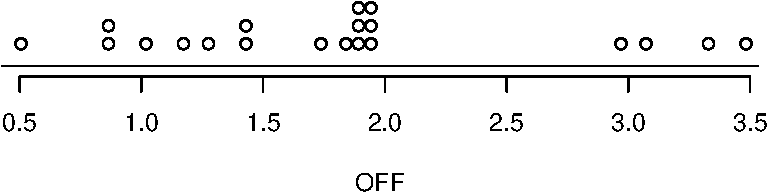
\includegraphics{pep1_files/figure-latex/unnamed-chunk-5-1.pdf}

\hypertarget{diagrama-de-puntos-para-visualizar-la-distribucion-de-los-puntajes-defensivos-de-los-equipos}{%
\subsection{1.2.2 Diagrama de puntos para visualizar la distribución de
los puntajes defensivos de los
equipos}\label{diagrama-de-puntos-para-visualizar-la-distribucion-de-los-puntajes-defensivos-de-los-equipos}}

\begin{Shaded}
\begin{Highlighting}[]
\KeywordTok{library}\NormalTok{(}\StringTok{"BHH2"}\NormalTok{)}
\KeywordTok{dotPlot}\NormalTok{(equipos}\OperatorTok{$}\NormalTok{DEF,}\DataTypeTok{xlab =} \StringTok{"OFF"}\NormalTok{)}
\end{Highlighting}
\end{Shaded}

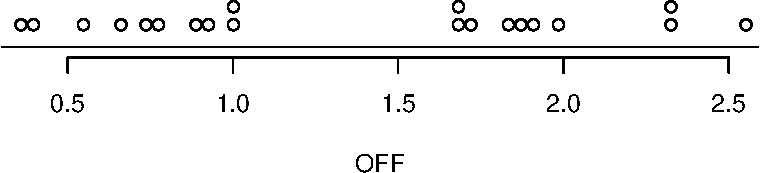
\includegraphics{pep1_files/figure-latex/unnamed-chunk-6-1.pdf}

\hypertarget{diagrama-de-puntos-para-visualizar-la-distribucion-de-los-puntajes-de-poder-adquisitivo-de-los-equipos}{%
\subsection{1.2.3 Diagrama de puntos para visualizar la distribución de
los puntajes de poder adquisitivo de los
equipos}\label{diagrama-de-puntos-para-visualizar-la-distribucion-de-los-puntajes-de-poder-adquisitivo-de-los-equipos}}

\begin{Shaded}
\begin{Highlighting}[]
\KeywordTok{library}\NormalTok{(}\StringTok{"BHH2"}\NormalTok{)}
\KeywordTok{dotPlot}\NormalTok{(equipos}\OperatorTok{$}\NormalTok{SPI,}\DataTypeTok{xlab =} \StringTok{"OFF"}\NormalTok{)}
\end{Highlighting}
\end{Shaded}

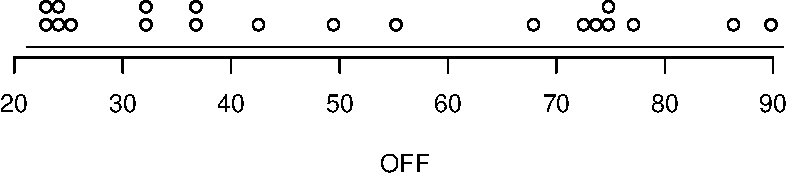
\includegraphics{pep1_files/figure-latex/unnamed-chunk-7-1.pdf}

\hypertarget{histogramas}{%
\subsubsection{1.3 Histogramas}\label{histogramas}}

\hypertarget{histograma-para-off}{%
\subsection{1.3.1 Histograma para OFF}\label{histograma-para-off}}

\begin{Shaded}
\begin{Highlighting}[]
\KeywordTok{library}\NormalTok{(}\StringTok{"ggplot2"}\NormalTok{)}
\end{Highlighting}
\end{Shaded}

\begin{verbatim}
## Registered S3 methods overwritten by 'ggplot2':
##   method         from 
##   [.quosures     rlang
##   c.quosures     rlang
##   print.quosures rlang
\end{verbatim}

\begin{Shaded}
\begin{Highlighting}[]
\NormalTok{grafico=}\KeywordTok{ggplot}\NormalTok{(equipos,}\KeywordTok{aes}\NormalTok{(equipos}\OperatorTok{$}\NormalTok{OFF)) }\CommentTok{# Gráfico y datos base}
\CommentTok{#Histograma (25 niveles) (colores- http://www.stat.columbia.edu/~tzheng/files/Rcolor.pdf)}
\NormalTok{grafico =}\StringTok{ }\NormalTok{grafico }\OperatorTok{+}\StringTok{ }\KeywordTok{geom_histogram}\NormalTok{(}\DataTypeTok{bins=}\DecValTok{25}\NormalTok{,}\DataTypeTok{fill=}\StringTok{"navajowhite"}\NormalTok{,}\DataTypeTok{color=}\StringTok{"orange3"}\NormalTok{)}
\NormalTok{grafico =}\StringTok{ }\NormalTok{grafico }\OperatorTok{+}\StringTok{ }\KeywordTok{theme_bw}\NormalTok{() }\CommentTok{# Visualización estándar en blanco y negro}
\NormalTok{grafico =}\StringTok{ }\NormalTok{grafico }\OperatorTok{+}\StringTok{ }\KeywordTok{ylab}\NormalTok{(}\StringTok{"Frecuencia absotula (equipos)"}\NormalTok{) }\OperatorTok{+}\StringTok{ }\KeywordTok{xlab}\NormalTok{(}\StringTok{"OFF"}\NormalTok{)}
\NormalTok{grafico =}\StringTok{ }\NormalTok{grafico }\OperatorTok{+}\StringTok{ }\KeywordTok{ggtitle}\NormalTok{(}\StringTok{"Histograma de OFF"}\NormalTok{)}
\KeywordTok{plot}\NormalTok{(grafico)}
\end{Highlighting}
\end{Shaded}

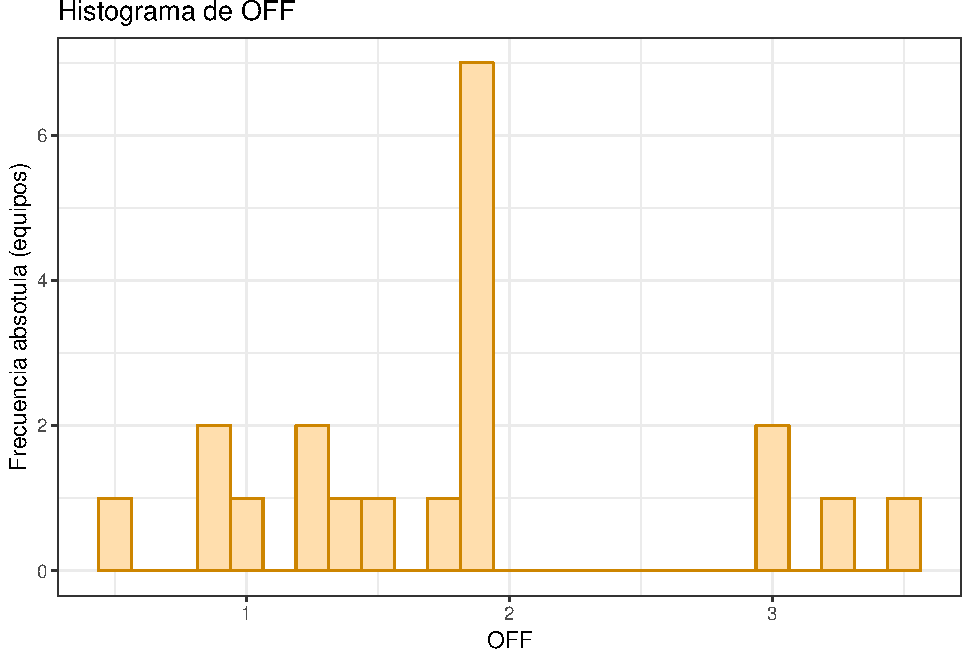
\includegraphics{pep1_files/figure-latex/unnamed-chunk-8-1.pdf}

\hypertarget{histograma-para-def}{%
\subsection{1.3.2 Histograma para DEF}\label{histograma-para-def}}

\begin{Shaded}
\begin{Highlighting}[]
\KeywordTok{library}\NormalTok{(}\StringTok{"ggplot2"}\NormalTok{)}
\NormalTok{grafico=}\KeywordTok{ggplot}\NormalTok{(equipos,}\KeywordTok{aes}\NormalTok{(equipos}\OperatorTok{$}\NormalTok{DEF)) }\CommentTok{# Gráfico y datos base}
\CommentTok{#Histograma (25 niveles) (colores- http://www.stat.columbia.edu/~tzheng/files/Rcolor.pdf)}
\NormalTok{grafico =}\StringTok{ }\NormalTok{grafico }\OperatorTok{+}\StringTok{ }\KeywordTok{geom_histogram}\NormalTok{(}\DataTypeTok{bins=}\DecValTok{25}\NormalTok{,}\DataTypeTok{fill=}\StringTok{"navajowhite"}\NormalTok{,}\DataTypeTok{color=}\StringTok{"orange3"}\NormalTok{)}
\NormalTok{grafico =}\StringTok{ }\NormalTok{grafico }\OperatorTok{+}\StringTok{ }\KeywordTok{theme_bw}\NormalTok{() }\CommentTok{# Visualización estándar en blanco y negro}
\NormalTok{grafico =}\StringTok{ }\NormalTok{grafico }\OperatorTok{+}\StringTok{ }\KeywordTok{ylab}\NormalTok{(}\StringTok{"Frecuencia absotula (equipos)"}\NormalTok{) }\OperatorTok{+}\StringTok{ }\KeywordTok{xlab}\NormalTok{(}\StringTok{"DEF"}\NormalTok{)}
\NormalTok{grafico =}\StringTok{ }\NormalTok{grafico }\OperatorTok{+}\StringTok{ }\KeywordTok{ggtitle}\NormalTok{(}\StringTok{"Histograma de DEF"}\NormalTok{)}
\KeywordTok{plot}\NormalTok{(grafico)}
\end{Highlighting}
\end{Shaded}

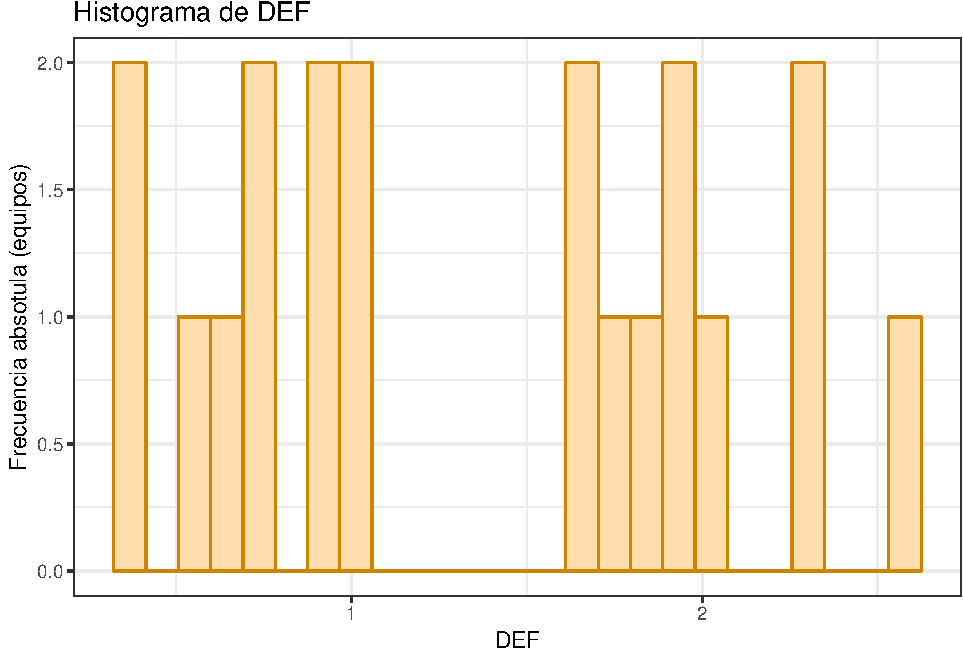
\includegraphics{pep1_files/figure-latex/unnamed-chunk-9-1.pdf}

\hypertarget{histograma-para-spi}{%
\subsection{1.3.3 Histograma para SPI}\label{histograma-para-spi}}

\begin{Shaded}
\begin{Highlighting}[]
\KeywordTok{library}\NormalTok{(}\StringTok{"ggplot2"}\NormalTok{)}
\NormalTok{grafico=}\KeywordTok{ggplot}\NormalTok{(equipos,}\KeywordTok{aes}\NormalTok{(equipos}\OperatorTok{$}\NormalTok{SPI)) }\CommentTok{# Gráfico y datos base}
\CommentTok{#Histograma (25 niveles) (colores- http://www.stat.columbia.edu/~tzheng/files/Rcolor.pdf)}
\NormalTok{grafico =}\StringTok{ }\NormalTok{grafico }\OperatorTok{+}\StringTok{ }\KeywordTok{geom_histogram}\NormalTok{(}\DataTypeTok{bins=}\DecValTok{25}\NormalTok{,}\DataTypeTok{fill=}\StringTok{"navajowhite"}\NormalTok{,}\DataTypeTok{color=}\StringTok{"orange3"}\NormalTok{)}
\NormalTok{grafico =}\StringTok{ }\NormalTok{grafico }\OperatorTok{+}\StringTok{ }\KeywordTok{theme_bw}\NormalTok{() }\CommentTok{# Visualización estándar en blanco y negro}
\NormalTok{grafico =}\StringTok{ }\NormalTok{grafico }\OperatorTok{+}\StringTok{ }\KeywordTok{ylab}\NormalTok{(}\StringTok{"Frecuencia absotula (equipos)"}\NormalTok{) }\OperatorTok{+}\StringTok{ }\KeywordTok{xlab}\NormalTok{(}\StringTok{"SPI"}\NormalTok{)}
\NormalTok{grafico =}\StringTok{ }\NormalTok{grafico }\OperatorTok{+}\StringTok{ }\KeywordTok{ggtitle}\NormalTok{(}\StringTok{"Histograma de SPI"}\NormalTok{)}
\KeywordTok{plot}\NormalTok{(grafico)}
\end{Highlighting}
\end{Shaded}

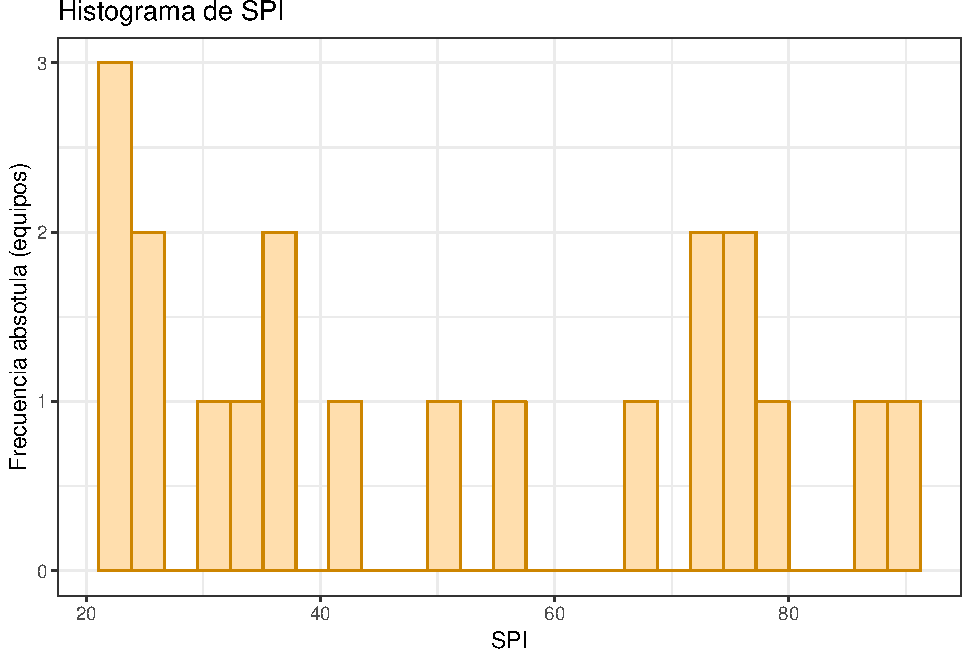
\includegraphics{pep1_files/figure-latex/unnamed-chunk-10-1.pdf}

\hypertarget{analisis-y-comparativa-entre-equipos-de-mejor-y-peor-rendimiento-y-nuestro-equipo-rayo-almendra}{%
\subsection{1.4 Análisis y comparativa entre equipos de mejor y peor
rendimiento y nuestro equipo (Rayo
Almendra)}\label{analisis-y-comparativa-entre-equipos-de-mejor-y-peor-rendimiento-y-nuestro-equipo-rayo-almendra}}

\hypertarget{minimo-y-maximo-de-puntaje-ofensivo-de-los-equipos}{%
\subsection{1.4.1 Mínimo y máximo de puntaje ofensivo de los
equipos}\label{minimo-y-maximo-de-puntaje-ofensivo-de-los-equipos}}

\begin{Shaded}
\begin{Highlighting}[]
\NormalTok{rango=}\KeywordTok{range}\NormalTok{(equipos}\OperatorTok{$}\NormalTok{OFF) }\CommentTok{# Rango mínimo y máximo de OFF de los equipos}
\NormalTok{rango}
\end{Highlighting}
\end{Shaded}

\begin{verbatim}
## [1] 0.48 3.48
\end{verbatim}

\hypertarget{el-puntaje-que-posee-el-equipo-con-mas-bajo-rendimiento-en-ofensiva-es-de-0.48-puntos-mientras-que-el-equipo-que-posee-el-mas-alto-puntaje-de-ofensiva-es-3.43.-el-equipo-rayo-almendra-tiene-un-puntaje-ofensivo-de-0.54-lo-que-lo-aleja-solamente-0.06-puntos-del-mas-bajo-y-una-diferencia-de-2.89-del-equipo-con-mejor-rendimiento-ofensivo-lo-que-posiciona-al-rayo-almendra-entre-el-20-con-mas-bajo-puntaje-de-la-tabla.}{%
\subsubsection{El puntaje que posee el equipo con más bajo rendimiento
en ofensiva es de 0.48 puntos, mientras que el equipo que posee el más
alto puntaje de ofensiva es 3.43. El equipo Rayo Almendra tiene un
puntaje ofensivo de 0.54, lo que lo aleja solamente 0.06 puntos del más
bajo y una diferencia de 2.89 del equipo con mejor rendimiento ofensivo,
lo que posiciona al Rayo Almendra entre el 20\% con más bajo puntaje de
la
tabla.}\label{el-puntaje-que-posee-el-equipo-con-mas-bajo-rendimiento-en-ofensiva-es-de-0.48-puntos-mientras-que-el-equipo-que-posee-el-mas-alto-puntaje-de-ofensiva-es-3.43.-el-equipo-rayo-almendra-tiene-un-puntaje-ofensivo-de-0.54-lo-que-lo-aleja-solamente-0.06-puntos-del-mas-bajo-y-una-diferencia-de-2.89-del-equipo-con-mejor-rendimiento-ofensivo-lo-que-posiciona-al-rayo-almendra-entre-el-20-con-mas-bajo-puntaje-de-la-tabla.}}

\hypertarget{minimo-y-maximo-de-puntaje-defensivo-de-los-equipos}{%
\subsection{1.4.2 Mínimo y máximo de puntaje defensivo de los
equipos}\label{minimo-y-maximo-de-puntaje-defensivo-de-los-equipos}}

\begin{Shaded}
\begin{Highlighting}[]
\NormalTok{rango=}\KeywordTok{range}\NormalTok{(equipos}\OperatorTok{$}\NormalTok{DEF) }\CommentTok{# Rango mínimo y máximo de DEF de los equipos}
\NormalTok{rango}
\end{Highlighting}
\end{Shaded}

\begin{verbatim}
## [1] 0.34 2.55
\end{verbatim}

\hypertarget{el-puntaje-minimo-obtenido-para-la-caracteristica-defensiva-de-los-equipos-es-de-0.26-mientras-el-maximo-es-de-2.51-puntos.-el-equipo-rayo-almendra-para-esta-categoria-tiene-un-puntaje-de-1.67-alejandolo-1.41-puntos-del-minimo-obtenido-y-0.84-del-puntaje-maximo-alcanzado-lo-que-posiciona-a-nuestro-equipo-entre-el-50-con-mejor-rendimiento-defensivo-del-campeonato.}{%
\subsubsection{El puntaje mínimo obtenido para la característica
defensiva de los equipos es de 0.26, mientras el máximo es de 2.51
puntos. El equipo Rayo Almendra, para esta categoría tiene un puntaje de
1.67, alejandolo 1.41 puntos del mínimo obtenido y 0.84 del puntaje
máximo alcanzado, lo que posiciona a nuestro equipo entre el 50\% con
mejor rendimiento defensivo del
campeonato.}\label{el-puntaje-minimo-obtenido-para-la-caracteristica-defensiva-de-los-equipos-es-de-0.26-mientras-el-maximo-es-de-2.51-puntos.-el-equipo-rayo-almendra-para-esta-categoria-tiene-un-puntaje-de-1.67-alejandolo-1.41-puntos-del-minimo-obtenido-y-0.84-del-puntaje-maximo-alcanzado-lo-que-posiciona-a-nuestro-equipo-entre-el-50-con-mejor-rendimiento-defensivo-del-campeonato.}}

\hypertarget{minimo-y-maximo-de-spi-de-los-equipos}{%
\subsection{1.4.3 Mínimo y máximo de SPI de los
equipos}\label{minimo-y-maximo-de-spi-de-los-equipos}}

\begin{Shaded}
\begin{Highlighting}[]
\NormalTok{rango=}\KeywordTok{range}\NormalTok{(equipos}\OperatorTok{$}\NormalTok{SPI) }\CommentTok{# Rango mínimo y máximo de SPI de los equipos}
\NormalTok{rango}
\end{Highlighting}
\end{Shaded}

\begin{verbatim}
## [1] 22.34 89.73
\end{verbatim}

\hypertarget{el-equipo-que-posee-el-minimo-spi-tiene-15.52-puntos-mientras-que-el-que-posee-el-maximo-puntaje-tiene-90.99-puntos.-el-equipo-rayo-almendra-tiene-para-esta-categoria-52.06-puntos-lo-que-lo-aleja-36.54-puntos-del-peor-y-38.93-puntos-del-mejor.-lo-que-posiciona-a-nuestro-equipo-entre-el-55-de-mejor-puntaje-en-spi-del-campeonato-y-perteneciendo-su-puntaje-a-un-35-del-total-del-espacio-muestral.}{%
\subsubsection{El equipo que posee el mínimo SPI tiene 15.52 puntos,
mientras que el que posee el máximo puntaje tiene 90.99 puntos. El
equipo Rayo Almendra tiene para esta categoría 52.06 puntos, lo que lo
aleja 36.54 puntos del peor y 38.93 puntos del mejor. Lo que posiciona a
nuestro equipo entre el 55\% de mejor puntaje en SPI del campeonato y
perteneciendo su puntaje a un 35\% del total del espacio
muestral.}\label{el-equipo-que-posee-el-minimo-spi-tiene-15.52-puntos-mientras-que-el-que-posee-el-maximo-puntaje-tiene-90.99-puntos.-el-equipo-rayo-almendra-tiene-para-esta-categoria-52.06-puntos-lo-que-lo-aleja-36.54-puntos-del-peor-y-38.93-puntos-del-mejor.-lo-que-posiciona-a-nuestro-equipo-entre-el-55-de-mejor-puntaje-en-spi-del-campeonato-y-perteneciendo-su-puntaje-a-un-35-del-total-del-espacio-muestral.}}

\hypertarget{generalmente-la-diferencia-para-las-categorias-entre-los-peores-y-mejores-rendimientos-es-la-siguiente}{%
\subsubsection{Generalmente la diferencia para las categorias entre los
peores y mejores rendimientos es la
siguiente:}\label{generalmente-la-diferencia-para-las-categorias-entre-los-peores-y-mejores-rendimientos-es-la-siguiente}}

\begin{itemize}
  \item El peor equipo tiene una diferencia de \textbf{\textit{2.95}} puntos del equipo con mejor ofensiva.
  \item El peor equipo tiene una diferencia de \textbf{\textit{2.25}} puntos del equipo con mejor defensiva.
  \item El peor equipo tiene una diferencia de \textbf{\textit{75.47}} puntos del equipo con mejor poder adquisitivo.
\end{itemize}

\hypertarget{analisis-de-equipos-aplicando-medidas-de-centralidad-media}{%
\subsection{1.5 Análisis de equipos aplicando medidas de centralidad
(Media)}\label{analisis-de-equipos-aplicando-medidas-de-centralidad-media}}

\hypertarget{media-de-off}{%
\subsection{1.5.1 Media de OFF}\label{media-de-off}}

\begin{Shaded}
\begin{Highlighting}[numbers=left,,]
\NormalTok{mediana_off =}\StringTok{ }\KeywordTok{median}\NormalTok{(equipos}\OperatorTok{$}\NormalTok{OFF)}
\KeywordTok{print}\NormalTok{(}\KeywordTok{paste}\NormalTok{(mediana_off))}
\end{Highlighting}
\end{Shaded}

\begin{verbatim}
## [1] "1.86"
\end{verbatim}

\hypertarget{el-equipo-rayo-almendra-tiene-un-puntaje-de-0.54-lo-que-lo-posiciona-por-debajo-de-la-puntuacion-media-para-la-caracteristica-ofensiva.}{%
\subsubsection{\texorpdfstring{El equipo Rayo Almendra tiene un puntaje
de \textbf{0.54}, lo que lo posiciona por debajo de la puntuación media
para la característica
ofensiva.}{El equipo Rayo Almendra tiene un puntaje de 0.54, lo que lo posiciona por debajo de la puntuación media para la característica ofensiva.}}\label{el-equipo-rayo-almendra-tiene-un-puntaje-de-0.54-lo-que-lo-posiciona-por-debajo-de-la-puntuacion-media-para-la-caracteristica-ofensiva.}}

\hypertarget{equipos-por-sobre-la-media-de-off}{%
\subsection{Equipos por sobre la Media de
(OFF)}\label{equipos-por-sobre-la-media-de-off}}

\begin{Shaded}
\begin{Highlighting}[numbers=left,,]
\KeywordTok{library}\NormalTok{(}\StringTok{"dplyr"}\NormalTok{,}\DataTypeTok{warn.conflicts =}\NormalTok{ F)}
\NormalTok{filtro1=}\KeywordTok{filter}\NormalTok{(equipos, OFF }\OperatorTok{>}\StringTok{ }\NormalTok{mediana_off)}
\NormalTok{filtro1=filtro1[}\KeywordTok{order}\NormalTok{(filtro1}\OperatorTok{$}\NormalTok{OFF , }\DataTypeTok{decreasing =} \OtherTok{TRUE}\NormalTok{),]}
\CommentTok{#kable(filtro1)}
\KeywordTok{kable}\NormalTok{(filtro1)}\OperatorTok
\KeywordTok{kable_styling}\NormalTok{(}\DataTypeTok{latex_options =} \StringTok{"striped"}\NormalTok{) }\CommentTok{# Aplicación de estilos a la tabla}
\end{Highlighting}
\end{Shaded}

\begin{table}[H]
\centering
\begin{tabular}{l|l|r|r|r}
\hline
  & EQUIPO & OFF & DEF & SPI\\
\hline
\rowcolor{gray!6}  3 & Cruz Maracuya & 3.48 & 1.69 & 68.10\\
\hline
7 & DC Ciruela & 3.31 & 2.33 & 77.49\\
\hline
\rowcolor{gray!6}  9 & Sociedad Frutilla & 3.06 & 2.55 & 86.89\\
\hline
10 & Jaguares de Higo & 2.95 & 0.93 & 37.16\\
\hline
\rowcolor{gray!6}  1 & Sport Limon & 1.93 & 0.38 & 22.34\\
\hline
5 & Alianza de Durazno & 1.93 & 0.55 & 22.50\\
\hline
\rowcolor{gray!6}  6 & Liga de Ajo & 1.92 & 1.83 & 72.36\\
\hline
2 & Nuevo Chirimoya & 1.90 & 1.91 & 36.78\\
\hline
\rowcolor{gray!6}  4 & Audax Rosa Mosqueta & 1.89 & 1.70 & 31.62\\
\hline
8 & New Coliflor & 1.89 & 0.34 & 32.64\\
\hline
\end{tabular}
\end{table}

\begin{Shaded}
\begin{Highlighting}[numbers=left,,]
\KeywordTok{paste}\NormalTok{(}\KeywordTok{count}\NormalTok{(filtro1)}\OperatorTok{$}\NormalTok{n, }\StringTok{"equipos por sobre la media OFF de un total de"}\NormalTok{, }\KeywordTok{count}\NormalTok{(equipos)}\OperatorTok{$}\NormalTok{n )}
\end{Highlighting}
\end{Shaded}

\begin{verbatim}
## [1] "10 equipos por sobre la media OFF de un total de 20"
\end{verbatim}

\hypertarget{media-de-def}{%
\subsection{1.5.2 Media de DEF}\label{media-de-def}}

\begin{Shaded}
\begin{Highlighting}[numbers=left,,]
\NormalTok{mediana_def =}\StringTok{ }\KeywordTok{median}\NormalTok{(equipos}\OperatorTok{$}\NormalTok{DEF)}
\KeywordTok{print}\NormalTok{(}\KeywordTok{paste}\NormalTok{(mediana_def))}
\end{Highlighting}
\end{Shaded}

\begin{verbatim}
## [1] "1.35"
\end{verbatim}

\hypertarget{el-equipo-rayo-almendra-para-la-puntuacion-de-defensiva-tiene-un-puntaje-de-1.67-lo-que-lo-posiciona-por-sobre-el-puntaje-medio-1.475.}{%
\subsubsection{\texorpdfstring{El equipo Rayo Almendra para la
puntuación de defensiva tiene un puntaje de \textbf{1.67}, lo que lo
posiciona por sobre el puntaje medio
(1.475).}{El equipo Rayo Almendra para la puntuación de defensiva tiene un puntaje de 1.67, lo que lo posiciona por sobre el puntaje medio (1.475).}}\label{el-equipo-rayo-almendra-para-la-puntuacion-de-defensiva-tiene-un-puntaje-de-1.67-lo-que-lo-posiciona-por-sobre-el-puntaje-medio-1.475.}}

\hypertarget{equipos-por-sobre-la-media-de-def}{%
\subsection{Equipos por sobre la Media de
(DEF)}\label{equipos-por-sobre-la-media-de-def}}

\begin{Shaded}
\begin{Highlighting}[numbers=left,,]
\KeywordTok{library}\NormalTok{(}\StringTok{"dplyr"}\NormalTok{,}\DataTypeTok{warn.conflicts =}\NormalTok{ F)}
\NormalTok{filtro2=}\KeywordTok{filter}\NormalTok{(equipos, DEF }\OperatorTok{>}\StringTok{ }\NormalTok{mediana_def)}
\NormalTok{filtro2=filtro2[}\KeywordTok{order}\NormalTok{(filtro2}\OperatorTok{$}\NormalTok{DEF, }\DataTypeTok{decreasing =} \OtherTok{TRUE}\NormalTok{),]}
\CommentTok{#kable(filtro2)}
\KeywordTok{kable}\NormalTok{(filtro2)}\OperatorTok
\KeywordTok{kable_styling}\NormalTok{(}\DataTypeTok{latex_options =} \StringTok{"striped"}\NormalTok{) }\CommentTok{# Aplicación de estilos a la tabla}
\end{Highlighting}
\end{Shaded}

\begin{table}[H]
\centering
\begin{tabular}{l|l|r|r|r}
\hline
  & EQUIPO & OFF & DEF & SPI\\
\hline
\rowcolor{gray!6}  10 & Sociedad Frutilla & 3.06 & 2.55 & 86.89\\
\hline
7 & DC Ciruela & 3.31 & 2.33 & 77.49\\
\hline
\rowcolor{gray!6}  9 & Rio Damasco & 1.03 & 2.32 & 89.73\\
\hline
4 & Independiente de  Platano & 1.26 & 1.99 & 74.49\\
\hline
\rowcolor{gray!6}  2 & Nuevo Chirimoya & 1.90 & 1.91 & 36.78\\
\hline
8 & Provincial Manzana & 0.84 & 1.89 & 23.85\\
\hline
\rowcolor{gray!6}  6 & Liga de Ajo & 1.92 & 1.83 & 72.36\\
\hline
1 & Puerto Pera & 1.83 & 1.73 & 55.03\\
\hline
\rowcolor{gray!6}  5 & Audax Rosa Mosqueta & 1.89 & 1.70 & 31.62\\
\hline
3 & Cruz Maracuya & 3.48 & 1.69 & 68.10\\
\hline
\end{tabular}
\end{table}

\begin{Shaded}
\begin{Highlighting}[numbers=left,,]
\KeywordTok{paste}\NormalTok{(}\KeywordTok{count}\NormalTok{(filtro2)}\OperatorTok{$}\NormalTok{n, }\StringTok{"equipos por sobre la media DEF de un total de"}\NormalTok{, }\KeywordTok{count}\NormalTok{(equipos)}\OperatorTok{$}\NormalTok{n )}
\end{Highlighting}
\end{Shaded}

\begin{verbatim}
## [1] "10 equipos por sobre la media DEF de un total de 20"
\end{verbatim}

\hypertarget{se-puede-observar-al-equipo-en-la-posicion-n9-de-la-tabla-de-equipos-sobre-la-media-en-def.}{%
\subsubsection{Se puede observar al equipo en la posición n°9 de la
tabla de equipos sobre la media en
DEF.}\label{se-puede-observar-al-equipo-en-la-posicion-n9-de-la-tabla-de-equipos-sobre-la-media-en-def.}}

\hypertarget{media-de-spi}{%
\subsection{Media de SPI}\label{media-de-spi}}

\begin{Shaded}
\begin{Highlighting}[numbers=left,,]
\NormalTok{mediana_spi =}\StringTok{ }\KeywordTok{median}\NormalTok{(equipos}\OperatorTok{$}\NormalTok{SPI)}
\KeywordTok{print}\NormalTok{(}\KeywordTok{paste}\NormalTok{(mediana_spi))}
\end{Highlighting}
\end{Shaded}

\begin{verbatim}
## [1] "45.885"
\end{verbatim}

\hypertarget{el-equipo-rayo-almendra-tiene-un-puntaje-de-52.06-para-spi-lo-que-lo-posiciona-sobre-la-media-la-cual-es-51.11.}{%
\subsubsection{El equipo Rayo Almendra tiene un puntaje de 52.06 para
SPI, lo que lo posiciona sobre la media la cual es
51.11.}\label{el-equipo-rayo-almendra-tiene-un-puntaje-de-52.06-para-spi-lo-que-lo-posiciona-sobre-la-media-la-cual-es-51.11.}}

\hypertarget{equipos-por-sobre-la-media-de-spi}{%
\subsection{Equipos por sobre la Media de
(SPI)}\label{equipos-por-sobre-la-media-de-spi}}

\begin{Shaded}
\begin{Highlighting}[numbers=left,,]
\KeywordTok{library}\NormalTok{(}\StringTok{"dplyr"}\NormalTok{,}\DataTypeTok{warn.conflicts =}\NormalTok{ F)}
\NormalTok{filtro3=}\KeywordTok{filter}\NormalTok{(equipos, SPI }\OperatorTok{>}\StringTok{ }\NormalTok{mediana_spi)}
\NormalTok{filtro3=filtro3[}\KeywordTok{order}\NormalTok{(filtro3}\OperatorTok{$}\NormalTok{SPI, }\DataTypeTok{decreasing =} \OtherTok{TRUE}\NormalTok{),]}
\CommentTok{#kable(filtro3)}
\KeywordTok{kable}\NormalTok{(filtro3)}\OperatorTok
\KeywordTok{kable_styling}\NormalTok{(}\DataTypeTok{latex_options =} \StringTok{"striped"}\NormalTok{) }\CommentTok{# Aplicación de estilos a la tabla}
\end{Highlighting}
\end{Shaded}

\begin{table}[H]
\centering
\begin{tabular}{l|l|r|r|r}
\hline
  & EQUIPO & OFF & DEF & SPI\\
\hline
\rowcolor{gray!6}  8 & Rio Damasco & 1.03 & 2.32 & 89.73\\
\hline
9 & Sociedad Frutilla & 3.06 & 2.55 & 86.89\\
\hline
\rowcolor{gray!6}  7 & DC Ciruela & 3.31 & 2.33 & 77.49\\
\hline
5 & AC Lucuma & 0.89 & 0.90 & 74.77\\
\hline
\rowcolor{gray!6}  3 & Independiente de  Platano & 1.26 & 1.99 & 74.49\\
\hline
6 & Atletico Mandarina & 1.45 & 0.66 & 74.15\\
\hline
\rowcolor{gray!6}  4 & Liga de Ajo & 1.92 & 1.83 & 72.36\\
\hline
2 & Cruz Maracuya & 3.48 & 1.69 & 68.10\\
\hline
\rowcolor{gray!6}  1 & Puerto Pera & 1.83 & 1.73 & 55.03\\
\hline
10 & Deportes Aceituna & 1.19 & 1.01 & 49.73\\
\hline
\end{tabular}
\end{table}

\begin{Shaded}
\begin{Highlighting}[numbers=left,,]
\KeywordTok{paste}\NormalTok{(}\KeywordTok{count}\NormalTok{(filtro3)}\OperatorTok{$}\NormalTok{n, }\StringTok{"equipos por sobre la media SPI de un total de"}\NormalTok{, }\KeywordTok{count}\NormalTok{(equipos)}\OperatorTok{$}\NormalTok{n )}
\end{Highlighting}
\end{Shaded}

\begin{verbatim}
## [1] "10 equipos por sobre la media SPI de un total de 20"
\end{verbatim}

\hypertarget{el-equipo-rayo-almendra-queda-en-la-posicion-n7-de-la-tabla-de-los-equipos-sobre-la-media-de-spi.}{%
\subsubsection{El equipo Rayo Almendra queda en la posición n°7 de la
tabla de los equipos sobre la media de
SPI.}\label{el-equipo-rayo-almendra-queda-en-la-posicion-n7-de-la-tabla-de-los-equipos-sobre-la-media-de-spi.}}

\hypertarget{equipos-por-sobre-la-media-de-off-media-de-def-y-media-de-spi}{%
\subsection{Equipos por sobre la Media de (OFF), Media de (DEF) y Media
de
(SPI)}\label{equipos-por-sobre-la-media-de-off-media-de-def-y-media-de-spi}}

\begin{Shaded}
\begin{Highlighting}[numbers=left,,]
\NormalTok{filtro_final=}\KeywordTok{filter}\NormalTok{(equipos, OFF }\OperatorTok{>}\StringTok{ }\NormalTok{mediana_off)}
\NormalTok{filtro_final=}\KeywordTok{filter}\NormalTok{(filtro_final, DEF }\OperatorTok{>}\StringTok{ }\NormalTok{mediana_def)}
\NormalTok{filtro_final=}\KeywordTok{filter}\NormalTok{(filtro_final, SPI }\OperatorTok{>}\StringTok{ }\NormalTok{mediana_spi)}
\CommentTok{#kable(filtro_final)}
\KeywordTok{kable}\NormalTok{(filtro_final)}\OperatorTok
\KeywordTok{kable_styling}\NormalTok{(}\DataTypeTok{latex_options =} \StringTok{"striped"}\NormalTok{) }\CommentTok{# Aplicación de estilos a la tabla}
\end{Highlighting}
\end{Shaded}

\begin{table}[H]
\centering
\begin{tabular}{l|r|r|r}
\hline
EQUIPO & OFF & DEF & SPI\\
\hline
\rowcolor{gray!6}  Cruz Maracuya & 3.48 & 1.69 & 68.10\\
\hline
Liga de Ajo & 1.92 & 1.83 & 72.36\\
\hline
\rowcolor{gray!6}  DC Ciruela & 3.31 & 2.33 & 77.49\\
\hline
Sociedad Frutilla & 3.06 & 2.55 & 86.89\\
\hline
\end{tabular}
\end{table}

\begin{Shaded}
\begin{Highlighting}[numbers=left,,]
\KeywordTok{paste}\NormalTok{(}\KeywordTok{count}\NormalTok{(filtro_final)}\OperatorTok{$}\NormalTok{n, }\StringTok{"equipos por sobre todas las medias de un total de"}\NormalTok{, }\KeywordTok{count}\NormalTok{(equipos)}\OperatorTok{$}\NormalTok{n )}
\end{Highlighting}
\end{Shaded}

\begin{verbatim}
## [1] "4 equipos por sobre todas las medias de un total de 20"
\end{verbatim}

\begin{Shaded}
\begin{Highlighting}[]
\CommentTok{#install.packages('gtools')}
\KeywordTok{library}\NormalTok{(}\StringTok{"gtools"}\NormalTok{)}
\KeywordTok{source}\NormalTok{(}\StringTok{"source/jugar_partidos.R"}\NormalTok{)}
\NormalTok{partidos=}\KeywordTok{jugar_partidos}\NormalTok{(equipos)}
\KeywordTok{head}\NormalTok{(partidos,}\DecValTok{40}\NormalTok{) }\CommentTok{# Muestra los primeros 20 partidos  }
\end{Highlighting}
\end{Shaded}

\begin{verbatim}
##                   EQ1                       EQ2 OFF1 DEF1  SPI1 OFF2 DEF2
## 1           AC Lucuma        Alianza de Durazno 0.89 0.90 74.77 1.93 0.55
## 2           AC Lucuma        Atletico Mandarina 0.89 0.90 74.77 1.45 0.66
## 3           AC Lucuma       Audax Rosa Mosqueta 0.89 0.90 74.77 1.89 1.70
## 4           AC Lucuma              Cerro Papaya 0.89 0.90 74.77 1.41 0.77
## 5           AC Lucuma             Cruz Maracuya 0.89 0.90 74.77 3.48 1.69
## 6           AC Lucuma                DC Ciruela 0.89 0.90 74.77 3.31 2.33
## 7           AC Lucuma         Deportes Aceituna 0.89 0.90 74.77 1.19 1.01
## 8           AC Lucuma Independiente de  Platano 0.89 0.90 74.77 1.26 1.99
## 9           AC Lucuma          Jaguares de Higo 0.89 0.90 74.77 2.95 0.93
## 10          AC Lucuma               Liga de Ajo 0.89 0.90 74.77 1.92 1.83
## 11          AC Lucuma              New Coliflor 0.89 0.90 74.77 1.89 0.34
## 12          AC Lucuma           Nuevo Chirimoya 0.89 0.90 74.77 1.90 1.91
## 13          AC Lucuma        Provincial Manzana 0.89 0.90 74.77 0.84 1.89
## 14          AC Lucuma               Puerto Pera 0.89 0.90 74.77 1.83 1.73
## 15          AC Lucuma            Real Membrillo 0.89 0.90 74.77 0.48 1.01
## 16          AC Lucuma               Rio Damasco 0.89 0.90 74.77 1.03 2.32
## 17          AC Lucuma                   San Uva 0.89 0.90 74.77 1.76 0.75
## 18          AC Lucuma         Sociedad Frutilla 0.89 0.90 74.77 3.06 2.55
## 19          AC Lucuma               Sport Limon 0.89 0.90 74.77 1.93 0.38
## 20 Alianza de Durazno                 AC Lucuma 1.93 0.55 22.50 0.89 0.90
## 21 Alianza de Durazno        Atletico Mandarina 1.93 0.55 22.50 1.45 0.66
## 22 Alianza de Durazno       Audax Rosa Mosqueta 1.93 0.55 22.50 1.89 1.70
## 23 Alianza de Durazno              Cerro Papaya 1.93 0.55 22.50 1.41 0.77
## 24 Alianza de Durazno             Cruz Maracuya 1.93 0.55 22.50 3.48 1.69
## 25 Alianza de Durazno                DC Ciruela 1.93 0.55 22.50 3.31 2.33
## 26 Alianza de Durazno         Deportes Aceituna 1.93 0.55 22.50 1.19 1.01
## 27 Alianza de Durazno Independiente de  Platano 1.93 0.55 22.50 1.26 1.99
## 28 Alianza de Durazno          Jaguares de Higo 1.93 0.55 22.50 2.95 0.93
## 29 Alianza de Durazno               Liga de Ajo 1.93 0.55 22.50 1.92 1.83
## 30 Alianza de Durazno              New Coliflor 1.93 0.55 22.50 1.89 0.34
## 31 Alianza de Durazno           Nuevo Chirimoya 1.93 0.55 22.50 1.90 1.91
## 32 Alianza de Durazno        Provincial Manzana 1.93 0.55 22.50 0.84 1.89
## 33 Alianza de Durazno               Puerto Pera 1.93 0.55 22.50 1.83 1.73
## 34 Alianza de Durazno            Real Membrillo 1.93 0.55 22.50 0.48 1.01
## 35 Alianza de Durazno               Rio Damasco 1.93 0.55 22.50 1.03 2.32
## 36 Alianza de Durazno                   San Uva 1.93 0.55 22.50 1.76 0.75
## 37 Alianza de Durazno         Sociedad Frutilla 1.93 0.55 22.50 3.06 2.55
## 38 Alianza de Durazno               Sport Limon 1.93 0.55 22.50 1.93 0.38
## 39 Atletico Mandarina                 AC Lucuma 1.45 0.66 74.15 0.89 0.90
## 40 Atletico Mandarina        Alianza de Durazno 1.45 0.66 74.15 1.93 0.55
##     SPI2 GEQ1 GEQ2
## 1  22.50    1    1
## 2  74.15    0    1
## 3  31.62    1    1
## 4  25.63    1    1
## 5  68.10    1    2
## 6  77.49    1    2
## 7  49.73    1    1
## 8  74.49    1    1
## 9  37.16    1    2
## 10 72.36    1    1
## 11 32.64    1    1
## 12 36.78    1    1
## 13 23.85    2    0
## 14 55.03    1    1
## 15 24.10    1    0
## 16 89.73    1    0
## 17 42.04    1    1
## 18 86.89    1    2
## 19 22.34    1    1
## 20 74.77    2    0
## 21 74.15    2    1
## 22 31.62    3    1
## 23 25.63    3    1
## 24 68.10    3    2
## 25 77.49    3    2
## 26 49.73    2    1
## 27 74.49    2    1
## 28 37.16    3    2
## 29 72.36    2    1
## 30 32.64    2    1
## 31 36.78    3    1
## 32 23.85    3    0
## 33 55.03    3    1
## 34 24.10    3    0
## 35 89.73    2    0
## 36 42.04    2    1
## 37 86.89    3    2
## 38 22.34    2    1
## 39 74.77    1    0
## 40 22.50    2    1
\end{verbatim}

\hypertarget{actividades-asumiendo-probabilidad-uniforme}{%
\subsection{1.6 Actividades Asumiendo probabilidad
uniforme}\label{actividades-asumiendo-probabilidad-uniforme}}

\hypertarget{cuantos-partidos-se-jugaron-formule-explique-y-resuelva-el-problema-considerando-los-conceptos-de-combinacionpermutacion.}{%
\subsubsection{¿Cuántos partidos se jugaron? Formule, explique y
resuelva el problema considerando los conceptos de
combinación/permutación.}\label{cuantos-partidos-se-jugaron-formule-explique-y-resuelva-el-problema-considerando-los-conceptos-de-combinacionpermutacion.}}

\hypertarget{ya-que-el-orde-de-los-partidos-si-importa-ya-que-se-juega-uno-de-ida-y-uno-de-vuelta-es-decir-2-partidos-por-par-de-equipos-se-utiliza-el-concepto-de-permutacion-en-donde-utilizando-la-formula}{%
\subsubsection{Ya que el orde de los partidos si importa, ya que se
juega uno de ida y uno de vuelta, es decir, 2 partidos por par de
equipos, se utiliza el concepto de permutación, en donde utilizando la
formula}\label{ya-que-el-orde-de-los-partidos-si-importa-ya-que-se-juega-uno-de-ida-y-uno-de-vuelta-es-decir-2-partidos-por-par-de-equipos-se-utiliza-el-concepto-de-permutacion-en-donde-utilizando-la-formula}}

\newcommand*{\Perm}[2]{{}^{#1}\!P_{#2}}

\({}^{n}\!P_{k}=\frac{n!}{(n-k)!}\)

\hypertarget{en-donde-n-es-la-cantidad-total-de-equipos-20-y-n-es-la-cantidad-de-partidos-para-dos-equipos-se-reflejara-el-resultado-de-el-total-de-permutaciones-del-campeonato.}{%
\subsubsection{en donde N es la cantidad total de equipos (20) y n es la
cantidad de partidos para dos equipos, se reflejará el resultado de el
total de permutaciones del
campeonato.}\label{en-donde-n-es-la-cantidad-total-de-equipos-20-y-n-es-la-cantidad-de-partidos-para-dos-equipos-se-reflejara-el-resultado-de-el-total-de-permutaciones-del-campeonato.}}

\begin{Shaded}
\begin{Highlighting}[]
\KeywordTok{library}\NormalTok{(gtools)}
\NormalTok{n =}\StringTok{ }\DecValTok{2} \CommentTok{# Cantidad de partidos a jugar por par de equipos}
\NormalTok{N =}\StringTok{ }\DecValTok{20} \CommentTok{# Cantidad de equipos}
\NormalTok{permutaciones=}\StringTok{ }\KeywordTok{nrow}\NormalTok{(}\KeywordTok{permutations}\NormalTok{(N,n))}
\KeywordTok{print}\NormalTok{(permutaciones)}
\end{Highlighting}
\end{Shaded}

\begin{verbatim}
## [1] 380
\end{verbatim}

\hypertarget{analizando-los-resultados-la-cantidad-de-partidos-a-jugar-fueron-380-considerando-que-por-cada-partido-existe-uno-de-ida-y-uno-de-vuelta.}{%
\subsubsection{Analizando los resultados, la cantidad de partidos a
jugar fueron 380, considerando que por cada partido existe uno de ida y
uno de
vuelta.}\label{analizando-los-resultados-la-cantidad-de-partidos-a-jugar-fueron-380-considerando-que-por-cada-partido-existe-uno-de-ida-y-uno-de-vuelta.}}

\hypertarget{cual-es-la-probabilidad-de-que-su-equipo-al-finalizar-el-torneo-sea-el-ganador}{%
\subsubsection{¿Cuál es la probabilidad de que su equipo al finalizar el
torneo sea el
ganador?}\label{cual-es-la-probabilidad-de-que-su-equipo-al-finalizar-el-torneo-sea-el-ganador}}

\hypertarget{por-distribucion-de-bernoulli-ya-que-queremos-medir-uan-variable-aleatoria-que-mide-la-cantidad-de-exito-de-salir-campeon-bajo-el-experimento-de-jugar-un-torneo-en-donde-los-equipos-tiene-solo-2-posibles-eventos-salir-campeon-o-no-salir-campeon-se-aplica-el-metodo-dbern-que-tendra-como-parametro-x-campeon1-y-p120.}{%
\subsubsection{\texorpdfstring{Por distribución de Bernoulli, ya que
queremos medir uan variable aleatoria, que mide la cantidad de éxito de
salir campéon bajo el experimento de jugar un torneo, en donde los
equipos tiene solo 2 posibles eventos, salir campeón o no salir campeón,
se aplica el método \textbf{dbern} que tendrá como parámetro X =
campéón(1) y
p=1/20.}{Por distribución de Bernoulli, ya que queremos medir uan variable aleatoria, que mide la cantidad de éxito de salir campéon bajo el experimento de jugar un torneo, en donde los equipos tiene solo 2 posibles eventos, salir campeón o no salir campeón, se aplica el método dbern que tendrá como parámetro X = campéón(1) y p=1/20.}}\label{por-distribucion-de-bernoulli-ya-que-queremos-medir-uan-variable-aleatoria-que-mide-la-cantidad-de-exito-de-salir-campeon-bajo-el-experimento-de-jugar-un-torneo-en-donde-los-equipos-tiene-solo-2-posibles-eventos-salir-campeon-o-no-salir-campeon-se-aplica-el-metodo-dbern-que-tendra-como-parametro-x-campeon1-y-p120.}}

\begin{Shaded}
\begin{Highlighting}[]
\CommentTok{#install.packages("Rlab")}
\KeywordTok{library}\NormalTok{(Rlab)}
\end{Highlighting}
\end{Shaded}

\begin{verbatim}
## 
## Attaching package: 'Rlab'
\end{verbatim}

\begin{verbatim}
## The following object is masked from 'package:dplyr':
## 
##     count
\end{verbatim}

\begin{verbatim}
## The following objects are masked from 'package:stats':
## 
##     dexp, dgamma, dweibull, pexp, pgamma, pweibull, qexp, qgamma,
##     qweibull, rexp, rgamma, rweibull
\end{verbatim}

\begin{Shaded}
\begin{Highlighting}[]
\KeywordTok{print}\NormalTok{(}\KeywordTok{dbern}\NormalTok{(}\DecValTok{1}\NormalTok{, }\DecValTok{1}\OperatorTok{/}\DecValTok{20}\NormalTok{, }\DataTypeTok{log =} \OtherTok{FALSE}\NormalTok{))}
\end{Highlighting}
\end{Shaded}

\begin{verbatim}
## [1] 0.05
\end{verbatim}

\hypertarget{la-probabilidad-de-que-el-equipo-rayo-almendra-salga-campeon-es-de-0.05}\label{la-probabilidad-de-que-el-equipo-rayo-almendra-salga-campeon-es-de-0.05}}

\hypertarget{por-distribucion-de-bernoulli-tenemos-x-cantidad-de-veces-que-existe-un-ganador1-ya-que-existen-20-equipos-el-espacio-muestral-es-de-20.-se-considera-exito-ganar-entonces-la-probabilidad-es-120.-se-considera-fracaso-no-ganar-entonces-q1-p-1-120-1920.}{%
\subsubsection{por distribución de bernoulli tenemos x = cantidad de
veces que existe un ganador(1); ya que existen 20 equipos, el espacio
muestral es de 20. Se considera éxito ganar, entonces la probabilidad es
1/20. Se considera fracaso no ganar entonces q=1-P = 1-(1/20) =
19/20.}\label{por-distribucion-de-bernoulli-tenemos-x-cantidad-de-veces-que-existe-un-ganador1-ya-que-existen-20-equipos-el-espacio-muestral-es-de-20.-se-considera-exito-ganar-entonces-la-probabilidad-es-120.-se-considera-fracaso-no-ganar-entonces-q1-p-1-120-1920.}}

\hypertarget{la-probabilidad-de-que-el-equipo-sea-ganador-es-x-1-entonces-px1-120119201-1-0.05-lo-que-nos-indica-que-tenemos-una-probabilidad-de-0.05-de-ganar.}{%
\subsubsection{La probabilidad de que el equipo sea ganador es x = 1
entonces P(x=1) = (1/20)\^{}1*(19/20)\^{}(1-1) = 0.05, lo que nos indica
que tenemos una probabilidad de 0.05\% de
ganar.}\label{la-probabilidad-de-que-el-equipo-sea-ganador-es-x-1-entonces-px1-120119201-1-0.05-lo-que-nos-indica-que-tenemos-una-probabilidad-de-0.05-de-ganar.}}

\hypertarget{cual-es-probabilidad-de-que-su-equipo-sea-campeon-del-torneo-3-veces-consecutivas}{%
\subsubsection{¿Cuál es probabilidad de que su equipo sea campeón del
torneo 3 veces
consecutivas?}\label{cual-es-probabilidad-de-que-su-equipo-sea-campeon-del-torneo-3-veces-consecutivas}}

\begin{Shaded}
\begin{Highlighting}[]
\KeywordTok{library}\NormalTok{(gtools)}
\NormalTok{n =}\StringTok{ }\DecValTok{2} \CommentTok{# Cantidad de partidos a jugar por par de equipos}
\NormalTok{N =}\StringTok{ }\DecValTok{20} \CommentTok{# Cantidad de equipos}
\NormalTok{permutaciones=}\StringTok{ }\KeywordTok{nrow}\NormalTok{(}\KeywordTok{permutations}\NormalTok{(N,n))}
\KeywordTok{print}\NormalTok{(permutaciones)}
\end{Highlighting}
\end{Shaded}

\begin{verbatim}
## [1] 380
\end{verbatim}

\hypertarget{cual-es-probabilidad-de-que-su-equipo-sea-campeon-del-torneo-3-veces-consecutivas}{%
\subsubsection{¿Cuál es probabilidad de que su equipo sea campeón del
torneo 3 veces
consecutivas?}\label{cual-es-probabilidad-de-que-su-equipo-sea-campeon-del-torneo-3-veces-consecutivas}}

\hypertarget{utilizando-distribucion-binomial-obtendremos-la-probabilidad-de-que-nuestro-equipo-salga-3-veces-campeon-de-forma-consecutiva.-aplicando-la-formula-de-distribucion-bonimial-en-donde-x-3-veces-que-se-busca-salir-campeon-n-3-cantidad-de-campeonatos-jugados-p-120-posibilidad-de-salir-campeon.-se-utiliza-metodo-dbinomxnp.}{%
\subsubsection{Utilizando distribución binomial obtendremos la
probabilidad de que nuestro equipo salga 3 veces campeón de forma
consecutiva. Aplicando la formula de Distribución bonimial en donde x =
3 (veces que se busca salir campeón), n = 3 (cantidad de campeonatos
jugados), p = 1/20 (posibilidad de salir campeón). Se utiliza método
dbinom(x,n,p).}\label{utilizando-distribucion-binomial-obtendremos-la-probabilidad-de-que-nuestro-equipo-salga-3-veces-campeon-de-forma-consecutiva.-aplicando-la-formula-de-distribucion-bonimial-en-donde-x-3-veces-que-se-busca-salir-campeon-n-3-cantidad-de-campeonatos-jugados-p-120-posibilidad-de-salir-campeon.-se-utiliza-metodo-dbinomxnp.}}

\begin{Shaded}
\begin{Highlighting}[]
\KeywordTok{print}\NormalTok{(}\KeywordTok{dbinom}\NormalTok{(}\DecValTok{3}\NormalTok{,}\DecValTok{3}\NormalTok{,}\FloatTok{0.05}\NormalTok{))}
\end{Highlighting}
\end{Shaded}

\begin{verbatim}
## [1] 0.000125
\end{verbatim}

\hypertarget{la-probabilidad-de-que-nuestro-equipo-salga-campeon-3-veces-consecutivas-es-de-0.000125}\label{la-probabilidad-de-que-nuestro-equipo-salga-campeon-3-veces-consecutivas-es-de-0.000125}}

\hypertarget{cual-es-la-probalidad-de-que-un-equipo-con-un-puntaje-de-ofensiva-off-sobre-la-media-no-sea-ganador-del-torneo}{%
\subsubsection{¿Cuál es la probalidad de que un equipo con un puntaje de
ofensiva (OFF) sobre la media NO sea ganador del
torneo?}\label{cual-es-la-probalidad-de-que-un-equipo-con-un-puntaje-de-ofensiva-off-sobre-la-media-no-sea-ganador-del-torneo}}

\hypertarget{ya-que-en-el-punto-1.5.1-tenemos-la-tabla-que-indica-los-equipos-por-sobre-la-media-de-off-nuestro-espacio-muestral-se-reduce-a-10-equipos-de-los-20-ya-que-se-aplico-un-filtro-sobre-la-totalidad.}{%
\subsubsection{Ya que en el punto 1.5.1 tenemos la tabla que indica los
equipos por sobre la media de OFF, nuestro espacio muestral se reduce a
10 equipos de los 20, ya que se aplicó un filtro sobre la
totalidad.}\label{ya-que-en-el-punto-1.5.1-tenemos-la-tabla-que-indica-los-equipos-por-sobre-la-media-de-off-nuestro-espacio-muestral-se-reduce-a-10-equipos-de-los-20-ya-que-se-aplico-un-filtro-sobre-la-totalidad.}}

\begin{Shaded}
\begin{Highlighting}[]
\KeywordTok{print}\NormalTok{(}\KeywordTok{dbern}\NormalTok{(}\DecValTok{0}\NormalTok{, }\DecValTok{1}\OperatorTok{/}\DecValTok{10}\NormalTok{, }\DataTypeTok{log =} \OtherTok{FALSE}\NormalTok{))}
\end{Highlighting}
\end{Shaded}

\begin{verbatim}
## [1] 0.9
\end{verbatim}

\hypertarget{la-probabilida-de-que-un-equipo-por-sobre-la-media-10-equipos-no-salga-campeon-es-de-un-0.9}{%
\subsubsection{La probabilida de que un equipo por sobre la media (10
equipos), no salga campeón es de un
0.9}\label{la-probabilida-de-que-un-equipo-por-sobre-la-media-10-equipos-no-salga-campeon-es-de-un-0.9}}

\hypertarget{finalizacion-del-campeonato}{%
\section{3.3 Finalización del
campeonato}\label{finalizacion-del-campeonato}}

\begin{Shaded}
\begin{Highlighting}[numbers=left,,]
\KeywordTok{source}\NormalTok{(}\StringTok{"source/resumen_torneo.R"}\NormalTok{) }\CommentTok{# Carga una función específica}
\NormalTok{tabla_resumen=}\KeywordTok{resumen_torneo}\NormalTok{(partidos) }\CommentTok{# Función para ver el resumen del torneo}
\KeywordTok{print}\NormalTok{(tabla_resumen[}\KeywordTok{c}\NormalTok{(}\DecValTok{1}\NormalTok{,}\DecValTok{5}\NormalTok{,}\DecValTok{6}\NormalTok{,}\DecValTok{7}\NormalTok{,}\DecValTok{8}\NormalTok{,}\DecValTok{9}\NormalTok{,}\DecValTok{10}\NormalTok{,}\DecValTok{11}\NormalTok{,}\DecValTok{12}\NormalTok{,}\DecValTok{13}\NormalTok{)])}\CommentTok{# Ver campos específicos de la tabla final}
\end{Highlighting}
\end{Shaded}

\begin{verbatim}
##                           EQ PPER PEMP PGAN PJUG GCON GFAV PTJE POS COND
## 6              Cruz Maracuya    3    6   29   38   65  117   93   1  GAN
## 10          Jaguares de Higo    4    6   28   38   60  112   90   2  ---
## 7                 DC Ciruela    5    9   24   38   76  105   81   3  ---
## 19         Sociedad Frutilla    5   10   23   38   78  100   79   4  ---
## 20               Sport Limon    9    6   23   38   55   79   75   5  ---
## 2         Alianza de Durazno    9    6   23   38   58   78   75   6  ---
## 3         Atletico Mandarina    5   12   21   38   40   59   75   7  ---
## 12              New Coliflor    8    8   22   38   51   78   74   8  ---
## 18                   San Uva    8   14   16   38   54   68   62   9  ---
## 5               Cerro Papaya   11   11   16   38   62   62   59  10  ---
## 11               Liga de Ajo   13   15   10   38   69   65   45  11  ---
## 15               Puerto Pera   16   13    9   38   77   63   40  12  ---
## 1                  AC Lucuma   13   18    7   38   44   34   39  13  ---
## 4        Audax Rosa Mosqueta   17   13    8   38   82   65   37  14  ---
## 13           Nuevo Chirimoya   17   13    8   38   82   65   37  15  ---
## 8          Deportes Aceituna   15   16    7   38   57   47   37  16  ---
## 9  Independiente de  Platano   27    8    3   38   72   39   17  17  ---
## 16            Real Membrillo   26   12    0   38   71   27   12  18  ---
## 17               Rio Damasco   32    6    0   38   75   26    6  19  DES
## 14        Provincial Manzana   34    4    0   38   88   27    4  20  DES
\end{verbatim}

\begin{itemize}
\tightlist
\item
  (PPER)
\item
  (PEMP)
\item
  (PGAN)
\item
  (PJUG)
\item
  (GCON)
\item
  (GFAV)
\item
  (PTJE)
\item
  (POS)
\item
  (COND)
\end{itemize}

\hypertarget{grafique-el-histograma}{%
\subsubsection{Grafique el histograma}\label{grafique-el-histograma}}

\begin{Shaded}
\begin{Highlighting}[]
\KeywordTok{library}\NormalTok{(}\StringTok{"ggplot2"}\NormalTok{)}
\NormalTok{grafico=}\KeywordTok{ggplot}\NormalTok{(tabla_resumen,}\KeywordTok{aes}\NormalTok{(tabla_resumen}\OperatorTok{$}\NormalTok{GCON)) }\CommentTok{# Gráfico y datos base}
\CommentTok{#Histograma (25 niveles) (colores- http://www.stat.columbia.edu/~tzheng/files/Rcolor.pdf)}
\NormalTok{grafico =}\StringTok{ }\NormalTok{grafico }\OperatorTok{+}\StringTok{ }\KeywordTok{geom_histogram}\NormalTok{(}\DataTypeTok{bins=}\DecValTok{20}\NormalTok{,}\DataTypeTok{fill=}\StringTok{"navajowhite"}\NormalTok{,}\DataTypeTok{color=}\StringTok{"orange3"}\NormalTok{)}
\NormalTok{grafico =}\StringTok{ }\NormalTok{grafico }\OperatorTok{+}\StringTok{ }\KeywordTok{theme_bw}\NormalTok{() }\CommentTok{# Visualización estándar en blanco y negro}
\NormalTok{grafico =}\StringTok{ }\NormalTok{grafico }\OperatorTok{+}\StringTok{ }\KeywordTok{ylab}\NormalTok{(}\StringTok{"Frecuencia absotula (equipos)"}\NormalTok{) }\OperatorTok{+}\StringTok{ }\KeywordTok{xlab}\NormalTok{(}\StringTok{"GCON"}\NormalTok{)}
\NormalTok{grafico =}\StringTok{ }\NormalTok{grafico }\OperatorTok{+}\StringTok{ }\KeywordTok{ggtitle}\NormalTok{(}\StringTok{"Histograma de Finalización del campeonato con mención en la columna GCON"}\NormalTok{)}
\KeywordTok{plot}\NormalTok{(grafico)}
\end{Highlighting}
\end{Shaded}

\begin{verbatim}
## Warning in grid.Call(C_textBounds, as.graphicsAnnot(x$label), x$x, x$y, :
## conversion failure on 'Histograma de Finalización del campeonato con
## mención en la columna GCON' in 'mbcsToSbcs': dot substituted for <cc>
\end{verbatim}

\begin{verbatim}
## Warning in grid.Call(C_textBounds, as.graphicsAnnot(x$label), x$x, x$y, :
## conversion failure on 'Histograma de Finalización del campeonato con
## mención en la columna GCON' in 'mbcsToSbcs': dot substituted for <81>
\end{verbatim}

\begin{verbatim}
## Warning in grid.Call(C_textBounds, as.graphicsAnnot(x$label), x$x, x$y, :
## conversion failure on 'Histograma de Finalización del campeonato con
## mención en la columna GCON' in 'mbcsToSbcs': dot substituted for <cc>
\end{verbatim}

\begin{verbatim}
## Warning in grid.Call(C_textBounds, as.graphicsAnnot(x$label), x$x, x$y, :
## conversion failure on 'Histograma de Finalización del campeonato con
## mención en la columna GCON' in 'mbcsToSbcs': dot substituted for <81>
\end{verbatim}

\begin{verbatim}
## Warning in grid.Call(C_textBounds, as.graphicsAnnot(x$label), x$x, x$y, :
## conversion failure on 'Histograma de Finalización del campeonato con
## mención en la columna GCON' in 'mbcsToSbcs': dot substituted for <cc>
\end{verbatim}

\begin{verbatim}
## Warning in grid.Call(C_textBounds, as.graphicsAnnot(x$label), x$x, x$y, :
## conversion failure on 'Histograma de Finalización del campeonato con
## mención en la columna GCON' in 'mbcsToSbcs': dot substituted for <81>
\end{verbatim}

\begin{verbatim}
## Warning in grid.Call(C_textBounds, as.graphicsAnnot(x$label), x$x, x$y, :
## conversion failure on 'Histograma de Finalización del campeonato con
## mención en la columna GCON' in 'mbcsToSbcs': dot substituted for <cc>
\end{verbatim}

\begin{verbatim}
## Warning in grid.Call(C_textBounds, as.graphicsAnnot(x$label), x$x, x$y, :
## conversion failure on 'Histograma de Finalización del campeonato con
## mención en la columna GCON' in 'mbcsToSbcs': dot substituted for <81>
\end{verbatim}

\begin{verbatim}
## Warning in grid.Call(C_textBounds, as.graphicsAnnot(x$label), x$x, x$y, :
## conversion failure on 'Histograma de Finalización del campeonato con
## mención en la columna GCON' in 'mbcsToSbcs': dot substituted for <cc>
\end{verbatim}

\begin{verbatim}
## Warning in grid.Call(C_textBounds, as.graphicsAnnot(x$label), x$x, x$y, :
## conversion failure on 'Histograma de Finalización del campeonato con
## mención en la columna GCON' in 'mbcsToSbcs': dot substituted for <81>
\end{verbatim}

\begin{verbatim}
## Warning in grid.Call(C_textBounds, as.graphicsAnnot(x$label), x$x, x$y, :
## conversion failure on 'Histograma de Finalización del campeonato con
## mención en la columna GCON' in 'mbcsToSbcs': dot substituted for <cc>
\end{verbatim}

\begin{verbatim}
## Warning in grid.Call(C_textBounds, as.graphicsAnnot(x$label), x$x, x$y, :
## conversion failure on 'Histograma de Finalización del campeonato con
## mención en la columna GCON' in 'mbcsToSbcs': dot substituted for <81>
\end{verbatim}

\begin{verbatim}
## Warning in grid.Call(C_textBounds, as.graphicsAnnot(x$label), x$x, x$y, :
## conversion failure on 'Histograma de Finalización del campeonato con
## mención en la columna GCON' in 'mbcsToSbcs': dot substituted for <cc>
\end{verbatim}

\begin{verbatim}
## Warning in grid.Call(C_textBounds, as.graphicsAnnot(x$label), x$x, x$y, :
## conversion failure on 'Histograma de Finalización del campeonato con
## mención en la columna GCON' in 'mbcsToSbcs': dot substituted for <81>
\end{verbatim}

\begin{verbatim}
## Warning in grid.Call.graphics(C_text, as.graphicsAnnot(x$label), x$x,
## x$y, : conversion failure on 'Histograma de Finalización del campeonato con
## mención en la columna GCON' in 'mbcsToSbcs': dot substituted for <cc>
\end{verbatim}

\begin{verbatim}
## Warning in grid.Call.graphics(C_text, as.graphicsAnnot(x$label), x$x,
## x$y, : conversion failure on 'Histograma de Finalización del campeonato con
## mención en la columna GCON' in 'mbcsToSbcs': dot substituted for <81>
\end{verbatim}

\includegraphics{pep1_files/figure-latex/unnamed-chunk-28-1.pdf}

\hypertarget{la-distribucion-normal-de-los-goles-en-contra-gcon}{%
\subsubsection{La distribución normal de los goles en contra
(GCON)}\label{la-distribucion-normal-de-los-goles-en-contra-gcon}}

\begin{Shaded}
\begin{Highlighting}[numbers=left,,]
\NormalTok{tabla_freq_tabla_resumen=}\KeywordTok{table.freq}\NormalTok{(}\KeywordTok{hist}\NormalTok{(tabla_resumen}\OperatorTok{$}\NormalTok{GCON,}\DataTypeTok{breaks =} \StringTok{"Sturges"}\NormalTok{,}\DataTypeTok{plot=}\OtherTok{FALSE}\NormalTok{))}\CommentTok{#Crea Tabla Freq. del resultado de los partidos}
\KeywordTok{kable}\NormalTok{(tabla_freq_tabla_resumen)}\OperatorTok\StringTok{ }\CommentTok{# Crea tabla de forma gráfica}
\KeywordTok{kable_styling}\NormalTok{(}\DataTypeTok{latex_options =} \StringTok{"striped"}\NormalTok{) }\CommentTok{# Aplicación de estilos a la tabla}
\end{Highlighting}
\end{Shaded}

\begin{table}[H]
\centering
\begin{tabular}{r|r|r|r|r|r|r}
\hline
Lower & Upper & Main & Frequency & Percentage & CF & CPF\\
\hline
\rowcolor{gray!6}  40 & 50 & 45 & 2 & 10 & 2 & 10\\
\hline
50 & 60 & 55 & 6 & 30 & 8 & 40\\
\hline
\rowcolor{gray!6}  60 & 70 & 65 & 3 & 15 & 11 & 55\\
\hline
70 & 80 & 75 & 6 & 30 & 17 & 85\\
\hline
\rowcolor{gray!6}  80 & 90 & 85 & 3 & 15 & 20 & 100\\
\hline
\end{tabular}
\end{table}

\hypertarget{cual-es-la-probabilidad-de-que-un-equipo-haya-recibido-entre-80-y-100-goles-empleando-el-histogramatabla-de-frecuencia.}{%
\subsubsection{¿Cuál es la probabilidad de que un equipo haya recibido
entre 80 y 100 goles empleando el histograma/tabla de
frecuencia?.}\label{cual-es-la-probabilidad-de-que-un-equipo-haya-recibido-entre-80-y-100-goles-empleando-el-histogramatabla-de-frecuencia.}}

\begin{Shaded}
\begin{Highlighting}[]
\CommentTok{#install.packages("Rlab")}
\KeywordTok{library}\NormalTok{(Rlab)}
\KeywordTok{print}\NormalTok{(}\KeywordTok{dbern}\NormalTok{(}\DecValTok{1}\NormalTok{, }\DecValTok{1}\OperatorTok{/}\DecValTok{5}\NormalTok{, }\DataTypeTok{log =} \OtherTok{FALSE}\NormalTok{))}
\end{Highlighting}
\end{Shaded}

\begin{verbatim}
## [1] 0.2
\end{verbatim}

\hypertarget{cual-es-la-probabilidad-de-que-un-equipo-haya-recibido-entre-80-y-100-goles-asumiendo-una-distribucion-normal}{%
\subsubsection{¿Cuál es la probabilidad de que un equipo haya recibido
entre 80 y 100 goles asumiendo una distribución
normal?}\label{cual-es-la-probabilidad-de-que-un-equipo-haya-recibido-entre-80-y-100-goles-asumiendo-una-distribucion-normal}}

\hypertarget{equipos-descendidos-contrataciones-y-venta-de-jugadores}{%
\section{3.4 Equipos descendidos, contrataciones y venta de
jugadores}\label{equipos-descendidos-contrataciones-y-venta-de-jugadores}}

\begin{Shaded}
\begin{Highlighting}[numbers=left,,]
\KeywordTok{source}\NormalTok{(}\StringTok{"source/actualizar_equipos.R"}\NormalTok{) }\CommentTok{# Cargar función específia}
\NormalTok{nombre=}\StringTok{"Rodrigo Vidal"} \CommentTok{# Emplee el nombre y apellido alumno 2}
\NormalTok{equipos_nuevos=}\KeywordTok{actualizar_equipos}\NormalTok{(nombre) }\CommentTok{# Función para actualizar equipos}
\KeywordTok{print}\NormalTok{(equipos_nuevos) }\CommentTok{# Mostrar equipos y parámetros}
\end{Highlighting}
\end{Shaded}

\begin{verbatim}
##                       EQUIPO  OFF  DEF   SPI COND
## 1                Puerto Pera 0.73 1.27 87.25  ANT
## 2                Sport Limon 2.10 0.96 73.03  ANT
## 3            Nuevo Chirimoya 0.66 1.03 30.46  ANT
## 4              Cruz Maracuya 0.54 0.28 67.30  ANT
## 5  Independiente de  Platano 0.42 2.09 33.85  ANT
## 6        Audax Rosa Mosqueta 3.10 0.43 54.44  ANT
## 7         Alianza de Durazno 1.34 2.32 69.94  ANT
## 8                Liga de Ajo 2.73 1.15 77.38  ANT
## 9             Real Membrillo 3.25 0.21 27.05  ANT
## 10                 AC Lucuma 1.71 0.62 84.60  ANT
## 11        Atletico Mandarina 2.43 1.21 69.28  ANT
## 12                DC Ciruela 0.64 1.35 31.60  ANT
## 13                   San Uva 2.71 2.35 83.47  ANT
## 14              New Coliflor 3.04 0.35 75.55  ANT
## 15              Cerro Papaya 1.68 1.68 41.51  ANT
## 16       Agrupacion Almendra 1.04 2.23 15.93  NUE
## 17               Liga de Uva 1.55 1.56 13.46  NUE
## 18         Sociedad Frutilla 2.05 0.53 89.34  ANT
## 19         Deportes Aceituna 0.86 1.20 55.65  ANT
## 20          Jaguares de Higo 0.61 0.77 39.35  ANT
\end{verbatim}

\begin{itemize}
\tightlist
\item
  Ataque (OFF)
\item
  Defensa (DEF)
\item
  Poder (SPI)
\item
  Indica si un equipo es nuevo (NUE) o antiguo (ANT) (COND)
\end{itemize}

\hypertarget{asumiendo-probalidad-uniforme-cual-es-la-probabilidad-de-que-un-equipo-no-salga-campeon-pero-tampoco-vaya-a-la-segunda-division}{%
\subsubsection{Asumiendo probalidad uniforme ¿Cuál es la probabilidad de
que un equipo NO salga campeón, pero tampoco vaya a la segunda
división?}\label{asumiendo-probalidad-uniforme-cual-es-la-probabilidad-de-que-un-equipo-no-salga-campeon-pero-tampoco-vaya-a-la-segunda-division}}

\hypertarget{caracterizar-los-parametros-de-los-equipos-off-def-y-spi-durante-el-torneo.}{%
\subsubsection{Caracterizar los parámetros de los equipos (OFF, DEF y
SPI) durante el
torneo.}\label{caracterizar-los-parametros-de-los-equipos-off-def-y-spi-durante-el-torneo.}}

\hypertarget{caracterizar-los-parametros-de-los-equipos-off-def-y-spi-una-vez-que-estos-se-actualizaron.}{%
\subsubsection{Caracterizar los parámetros de los equipos (OFF, DEF y
SPI) una vez que éstos se
actualizaron.}\label{caracterizar-los-parametros-de-los-equipos-off-def-y-spi-una-vez-que-estos-se-actualizaron.}}

\hypertarget{con-los-resultados-anteriores-establezca-una-comparacion-para-estas-tres-variables-durante-clase-1-y-despues-del-torneo-clase-2.-apoye-la-comparacion-empleando-graficos-de-cajas.}{%
\subsubsection{Con los resultados anteriores establezca una comparación
para estas tres variables durante (clase 1) y después del torneo (clase
2). Apoye la comparación empleando gráficos de
cajas.}\label{con-los-resultados-anteriores-establezca-una-comparacion-para-estas-tres-variables-durante-clase-1-y-despues-del-torneo-clase-2.-apoye-la-comparacion-empleando-graficos-de-cajas.}}

\hypertarget{si-su-equipo-no-descendio-compare-sus-caracteristicas-al-jugar-el-torneo-y-en-la-actualidad.}{%
\subsubsection{Si su equipo no descendió: compare sus características al
jugar el torneo y en la
actualidad.}\label{si-su-equipo-no-descendio-compare-sus-caracteristicas-al-jugar-el-torneo-y-en-la-actualidad.}}


\end{document}
